%------------------------------------------------------------------------------
\newpage
\section{UE 2: Elementarsignale- und Operationen, LTI-System Eigenschaften, Faltung}
\label{sec:ue2_faltung}

Wir müssen uns zunächst mit den zeitkontinuierlichen Elementarsignalen vertraut
machen, siehe \verb|fundamental_signals_CT.pdf| im StudIP unter Formelsammlung.

Diese sind
\begin{itemize}
  \item Exponentialfunktion
  $\e^{s_0 \, t}$ mit $s=\sigma_0 + \im\omega_0, s_0\in\mathbb{C}, \sigma_0\in\mathbb{R}, \omega_0\in\mathbb{R}$
  \item Rechtecksignal $\mathrm{rect}(t)$ (Konvention: Fläche 1)
  \item Dreiecksignal $\mathrm{tri}(t)$  (Konvention: Fläche 1)
  \item Spaltfunktion $\mathrm{sinc}(t):=\frac{\sin t}{t}$
  \item Sprungfunktion $\epsilon(t)$
  \item Vorzeichenfunktion $\mathrm{sgn}(t)$
  \item Dirac Impuls $\delta(t)$
  \item Dirac Impuls Kamm $\Sha$(t)
\end{itemize}
\red{TBD mit tikz / pgfplots}








\newpage
\subsection{Signaloperationen: Verschiebung und Skalierung}
\label{sec:42DE8C69F7}
\begin{Ziel}
Es ist wichtig, dass wir uns für die Zeitfunktion $f(t)$
die Operationen
Zeitverschiebung,
Zeitskalierung und die Amplitudenskalierung, also
$A \cdot f(\left[t-\tau\right]\cdot \theta)$ mit $A,\tau,\theta\in\mathbb{R}$
klarmachen.
%
Wie man so schön sagt, müssen wir das für SigSys im Schlaf beherrschen.
\end{Ziel}
\textbf{Aufgabe} {\tiny 42DE8C69F7}: Stellen Sie
{$x(t) = \frac{3}{4} \cdot \mathrm{rect}(\frac{1}{3} t-\frac{1}{2})$}
grafisch dar.
\begin{Werkzeug}
Für
\begin{equation}
A \cdot f(\left[t-\tau\right]\cdot \theta)  \qquad A,\tau,\theta\in\mathbb{R}
\end{equation}
gilt
\begin{itemize}
  \item Zeitverschiebung mit
  $\tau$: für $\tau>0$ verzögert, rechtsverschoben; für $\tau<0$ vorauseilend, linksverschoben
  \item Zeitskalierung mit $\theta$: für $\theta>1$ Stauchung; für $0<\theta<1$ Streckung
  \item Amplitudenskalierung mit $A$: für $0<|A|<1$ Stauchung, für $|A|>1$ Streckung
  \item (für $A<0$ zusätzlich noch Invertieren der Signalpolarität)
  \item (für $\theta<0$ zusätzlich noch Invertieren des Zeitverlaufs)
\end{itemize}
\end{Werkzeug}
\begin{Ansatz}
Es ist sinnvoll, das Signal in die Darstellung
\begin{equation}
x(t) = \frac{3}{4} \cdot \mathrm{rect}(\left[t-\frac{3}{2}\right]\cdot \frac{1}{3})
\end{equation}
umzuformen, weil dann $t$ ohne Vorfaktor und so wie obige Formel.
Dann lässt sich Zeitverschiebung und Zeitskalierung
getrennt und nacheinander abarbeiten. Hier also zunächst Zeitverzögerung um
$\frac{3}{2}$ und dann zeitliche Streckung (das Signal wird 'langsamer' bzw.
braucht über die Zeit länger) mit $\frac{1}{3}$.
%
Zum Schluss noch die Amplitudenstauchung auf Amplitude $1 \cdot \frac{3}{4}$.
%
Es ist empfehlenswert, sich das kochrezeptartig anzugewöhnen, bis es sitzt.

Bei einem cos()-Signal leuchtet uns die zeitliche Streckung, Stauchung vielleicht
intuitiv ein: ausgehend von $\cos(t)$ schwingt $\cos(2\,t)$ schneller, das ist eine
zeitliche Stauchung.
%
Jedoch ausgehend von $\cos(t)$ schwingt $\cos(\frac{1}{2}\,t)$
langsamer, das ist dann eine zeitliche Streckung.

Machen wir uns klar, dass wir auch eine Verschiebung des Signals bezüglich der
Ordinate vornehmen können. Das heißt wir manipulieren den Gleichanteil.
%
Signale mit Gleichanteil werden in den meisten signallastigen
Ingenieursdisziplinen vermieden, weil man den Gleichanteil schlecht
(elektrische Dauerlast, Wärme) oder gar nicht (z.B. Gleichstrom über Luft?!)
übertragen kann.
%
Wir benutzen das daher in den SigSys-UE seltener.

\end{Ansatz}
%\begin{ExCalc}
%\end{ExCalc}
\begin{Loesung}
Das Signal ist in \fig{fig:42DE8C69F7}d dargestellt. Der Lösungsweg folgt von
\fig{fig:42DE8C69F7}a zu \fig{fig:42DE8C69F7}d.

Eine gute Kontrollmöglichkeit bietet Wolfram Alpha
\url{https://www.wolframalpha.com/}.
Nachdem wir uns vergewissert haben, dass die Rechteckfunktion dort ähnlich definiert
ist (Breite, Höhe, Fläche ist jeweils 1), können wir
\verb|3/4*rect(1/3*t-1/2)| eingeben und bekommen eine analytische und grafische
Lösung von Wolfram Alpha angeboten.
Hinweis: die Sprungfunktion erhalten wir mit \verb|step(t)|
und die Dreieckfunktion mit \verb|tri(t)|, damit können wir eigene einfache
Experimente zur Signalskalierung und -verschiebung machen.
%
Das sollten wir in jedem Fall mal machen in einer Mußestunde!

%Mit UE 1.1 aus dem SS2019 können wir noch mehr üben.
\end{Loesung}

\begin{figure*}[h!]
\centering
\begin{subfigure}{0.45\textwidth}
\begin{tikzpicture}
\begin{axis}[
width=1\textwidth,
height=0.5\textwidth,
domain=-4:4,
samples=50,
legend pos=outer north east,
xlabel = {t},
%ylabel = {x(t)},
title = {$x(t) = \mathrm{rect}(t)$},
xmin=-4, xmax=4,
ymin=-0.1, ymax=1.1,
xtick={-4,-3,-2,-1,0,1,2,3,4},
ytick={0,0.5,1,1.5,2},
ymajorgrids=true,
xmajorgrids=true
]
\addplot[mark=None, color=C0, ultra thick]
coordinates {(-4,0)(-1/2,0)(-1/2,1)(1/2,1)(1/2,0)(4,0)};
\end{axis}
\end{tikzpicture}
\caption{Elementarsignal Rechteckfunktion.}
%\label{fig:}
\end{subfigure}
%
\begin{subfigure}{0.45\textwidth}
\begin{tikzpicture}
\begin{axis}[
width=1\textwidth,
height=0.5\textwidth,
domain=-4:4,
samples=50,
legend pos=outer north east,
xlabel = {t},
%ylabel = {x(t)},
title = {$x(t) = \mathrm{rect}(t-\frac{3}{2})$},
xmin=-4, xmax=4,
ymin=-0.1, ymax=1.1,
xtick={-4,-3,-2,-1,0,1,2,3,4},
ytick={0,0.5,1,1.5,2},
ymajorgrids=true,
xmajorgrids=true
]
\addplot[mark=None, color=C0, ultra thick]
coordinates {(-4,0)(1,0)(1,1)(2,1)(2,0)(4,0)};
\end{axis}
\end{tikzpicture}
\caption{Zeit\textbf{verzögerung}.}
%\label{fig:}
\end{subfigure}


\begin{subfigure}{0.45\textwidth}
\begin{tikzpicture}
\begin{axis}[
width=1\textwidth,
height=0.5\textwidth,
domain=-4:4,
samples=50,
legend pos=outer north east,
xlabel = {t},
%ylabel = {x(t)},
title = {$x(t) = \mathrm{rect}(\left[t-\frac{3}{2}\right]\cdot \frac{1}{3}) = \mathrm{rect}( \frac{t}{3} - \frac{1}{2})$},
xmin=-4, xmax=4,
ymin=-0.1, ymax=1.1,
xtick={-4,-3,-2,-1,0,1,2,3,4},
ytick={0,0.5,1,1.5,2},
ymajorgrids=true,
xmajorgrids=true
]
\addplot[mark=None, color=C0, ultra thick]
coordinates {(-4,0)(0,0)(0,1)(3,1)(3,0)(4,0)};
\end{axis}
\end{tikzpicture}
\caption{Zeitverzögerung und -\textbf{streckung}.}
%\label{fig:}
\end{subfigure}
%
\begin{subfigure}{0.45\textwidth}
\begin{tikzpicture}
\begin{axis}[
width=1\textwidth,
height=0.5\textwidth,
domain=-4:4,
samples=50,
legend pos=outer north east,
xlabel = {t},
%ylabel = {x(t)},
title = {$x(t) = \frac{3}{4} \cdot \mathrm{rect}(\left[t-\frac{3}{2}\right]\cdot \frac{1}{3})$},
xmin=-4, xmax=4,
ymin=-0.1, ymax=1.1,
xtick={-4,-3,-2,-1,0,1,2,3,4},
ytick={0,0.5,1,1.5,2},
ymajorgrids=true,
xmajorgrids=true
]
\addplot[mark=None, color=C0, ultra thick]
coordinates {(-4,0)(0,0)(0,3/4)(3,3/4)(3,0)(4,0)};
\end{axis}
\end{tikzpicture}
\caption{Zeitverzögerung/-streckung, \textbf{Amplitudenstauchung}.}
%\label{fig:}
\end{subfigure}
%
%
%
\caption{Skizzenfahrplan für Aufgabe \ref{sec:42DE8C69F7}.
\red{TBD: ipnyb}}
\label{fig:42DE8C69F7}
\end{figure*}





\newpage
\subsection{Ableitung eines Cosinus-Signalausschnitts}
\label{sec:114F06AFAA}
\begin{Ziel}
Wir wollen ein paar prototypische
Rechenmuster der SigSys kennenlernen. Dabei begegnen uns neben ganz normalem
Mathematik-Tools ein paar SigSys-Eigenheiten, die wir in den ersten Vorlesungen und Übungen
erarbeiten, also Standardsignale und deren Zusammenhänge und Eigenschaften.
\end{Ziel}
\textbf{Aufgabe} {\tiny 114F06AFAA}:
Gegeben ist das skizzierte Signal $x(t)$. Finden Sie einen analytisch geschlossenen
Ausdruck für $x(t)$ mit Hilfe von Elementarsignalen. Berechnen Sie die zeitliche
Ableitung $x'(t)$ und stellen Sie diese grafisch dar.
\begin{center}
\begin{tikzpicture}[scale=0.8]
\def \xmin {-4}
\def \xmax {4.2}
\def \ymin {-1}
\def \ymax {1.5}
\draw[->] (\xmin-0.1 ,0) -- (\xmax+0.1,0) node[below]{$t$};
\draw[->] (0,\ymin-0.1) -- (0,\ymax+0.1) node[left]{$x(t)$};
\foreach \x in {\xmin,...,3}{\draw (\x,0.05) -- (\x,-0.05);}
\draw (0.05,-1) -- (-0.05,-1);
\draw (0.05,1) -- (-0.05,1) node[left]{\small $1$};
\draw(2,0) node[below]{\small $2$};
\begin{scope}
\draw[C0, ultra thick, domain=-2:2,variable=\t,samples=100,smooth] plot(\t,{ cos (4*pi*\t r)});
\draw[C0, ultra thick] (-4,0) -- (-2,0);
\draw[C0, ultra thick] (2,0) -- (4,0);
\draw[C0, dashed, thin] (2,0) -- (2,1);
\draw[C0, dashed, thin] (-2,0) -- (-2,1);
\end{scope}
\end{tikzpicture}
\end{center}

\begin{Werkzeug}
Rechteckfunktion, Skalierung, Zerlegung in Sprungfunktionen, Ableitung

Ausblendeigenschaft / Austasteigenschaft des Dirac-Impulses,
was ja eigentlich eher eine Definition, anstatt eine Eigenschaft ist (siehe Übung~\ref{sec:ue1_intro} (1))
\begin{equation}
\int\limits_{-\infty}^{+\infty} \delta(t-\tau) \cdot f(t) \, \fsd t \stackrel{\mathrm{def}}= f(\tau)
\end{equation}

Multiplikationseigenschaft des Dirac-Impulses
\begin{align}
&\delta(t-\tau) f(t) = \delta(t-\tau) f(\tau)\\
&\delta(t) f(t) = \delta(t) f(0) \qquad \text{speziell für} \qquad \tau=0
\end{align}

\end{Werkzeug}
\begin{Ansatz}
Typische SigSys-Denke: Zeitlich begrenzten Cosinus herstellen indem wir mit der
Rechteckfunktion einen Teil ausschneiden. Dann Mathematik betreiben.
\end{Ansatz}
\begin{ExCalc}
Vier Schwingungen pro 2 Sekunden, also Frequenz $f=2$ Hz, also Kreisfrequenz
$\omega=2\pi\cdot 2 = 4\pi$ rad/s, also $\cos(4\pi t)$ (wir haben zeitlich gestaucht)
der nur zwischen $-2 < t < +2$ schwingt. Wir können den Cos dafür mit einer
geeigneten Rechteckfunktion multiplizieren.

Die benötigte Rechteckfunktion muss axialsymmetrisch sein, d.h. es ist keine
Zeitverschiebung involviert.
Die benötigte Rechteckfunktion muss breiter sein, als das Standardsignal
$\mathrm{rect}(t)$, d.h. es ist eine zeitliche Streckung erforderlich.
Breite von $\mathrm{rect}(t)$ ist 1 (hat auch Fläche 1!), wir brauchen aber
Breite 4, daher $\mathrm{rect}(t\cdot \frac{1}{4})$ (zur Erinnerung:
die Funktion soll sich bei Streckung langsamer über der Zeit ändern, daher
Skalierungsfaktor kleiner 1)

Daher kann das Signal als
\begin{align}
x(t) = \cos(4\pi t) \cdot \mathrm{rect}(\frac{t}{4})\\
\end{align}
darstellt werden. Kurzer Check bei Wolfram Alpha bestätigt, dass wir richtig
gerechnet haben.

Für die Zeitableitung
\begin{align}
\frac{\fsd }{\fsd t} x(t) =
\frac{\fsd }{\fsd t} \cos(4\pi t) \cdot \mathrm{rect}(\frac{t}{4})\\
\end{align}
benötigen wir nun die Produkt- und Kettenregel, sowie die Ableitung des Rechtecksignals.

Wir können das Rechtecksignal als Überlagerung von zwei Sprungfunktionen darstellen,
nämlich
\begin{equation}
\mathrm{rect}(\frac{t}{4}) = \epsilon(t+2) -\epsilon(t-2),
\end{equation}
was in der Grafik unten visualisiert ist. Zu besseren Übersichtlichkeit wurden die
Funktionen minimal verschoben/skaliert, damit wir auch bei eigentlicher
Überlappung sehen, wie sie verlaufen. Das Prinzip sollte erkennbar sein.
%
\begin{center}
\begin{tikzpicture}
\begin{axis}[
width=0.5\textwidth,
height=0.3\textwidth,
domain=-4:4,
samples=50,
legend pos=outer north east,
xlabel = {t},
%ylabel = {x(t)},
title = {Rechteckfunktion aus zwei Sprungfunktionen},
xmin=-4, xmax=4,
ymin=-1.1, ymax=1.1,
xtick={-4,-3,-2,-1,0,1,2,3,4},
ytick={-1,-0.5,0,0.5,1},
ymajorgrids=true,
xmajorgrids=true
]
\addplot[mark=None, color=C1, ultra thick]
coordinates {(-4,0.05)(-2,0.05)(-2,1)(4,1)};
\addplot[mark=None, color=C2, ultra thick]
coordinates {(-4,-0.05)(2,-0.05)(2,-1)(4,-1)};
\addplot[mark=None, color=C0, ultra thick]
coordinates {(-4,0)(-1.95,0)(-1.95,0.95)(2,0.95)(2,0)(4,0)};
\legend{$+\epsilon(t+2)$ (vorauseilend),$-\epsilon(t-2)$ (verzögert),$+\epsilon(t+2)-\epsilon(t-2)=\mathrm{rect}(t\cdot\frac{1}{4})$}
\end{axis}
\end{tikzpicture}
\end{center}

Nun brauchen wir folgende wichtige Erkenntnis (die nur indirekt in der Formelsammlung
steht, nämlich bei den Korrespondenzen zur Laplace Transformation) und in
\fig{fig:114F06AFAA} veranschaulicht ist
\begin{equation}
  \epsilon(t)' = \delta(t)
\end{equation}

Damit können wir jetzt ableiten.

Also, zunächst die Zerlegung der Rechteckfunktion in zwei Sprungfunktionen
\begin{align}
\frac{\fsd }{\fsd t} x(t) =
\frac{\fsd }{\fsd t} \cos(4\pi t) \cdot \left( \epsilon(t+2) -\epsilon(t-2)\right)=\\
\frac{\fsd }{\fsd t} \cos(4\pi t) \epsilon(t+2)
- \frac{\fsd }{\fsd t} \cos(4\pi t) \epsilon(t-2)
\end{align}

Ausformulieren bringt
\begin{align}x'(t)=
+ \cos(4\pi t)' \epsilon(t+2) + \cos(4\pi t) \epsilon(t+2)'
- \cos(4\pi t)' \epsilon(t-2) - \cos(4\pi t) \epsilon(t-2)'
\end{align}
\begin{align}x'(t)=
- 4\pi\sin(4\pi t) \epsilon(t+2) + \cos(4\pi t) \delta(t+2)
+ 4\pi\sin(4\pi t) \epsilon(t-2) - \cos(4\pi t) \delta(t-2)
\end{align}
Umsortieren, damit wir aus den Sprüngen wieder eine Rechteckfunktion machen können
(was natürlich nicht immer geht, hier aber zum Glück, weil...?)
\begin{align}x'(t)=
- 4\pi\sin(4\pi t) (\epsilon(t+2) - \epsilon(t-2))
+ \cos(4\pi t) \delta(t+2)
- \cos(4\pi t) \delta(t-2)
\end{align}
\begin{align}x'(t)=
- 4\pi\sin(4\pi t) \mathrm{rect}(\frac{t}{4})
+ \cos(4\pi t) \delta(t+2)
- \cos(4\pi t) \delta(t-2)
\end{align}
Mit der Multiplikationseigenschaft des Dirac Impulses
\begin{align}
\delta(t-\tau) f(t) = \delta(t-\tau) f(\tau)
\end{align}
finden wir vereinfachte Ausdrücke
\begin{align}
- \delta(t-2) \cos(4\pi t) = - \delta(t-2) \cos(4\pi \cdot 2) = - \delta(t-2)\\
+ \delta(t+2) \cos(4\pi t) = + \delta(t-(-2)) \cos(4\pi \cdot (-2)) = + \delta(t+2)
\end{align}
und damit wird
\begin{align}x'(t)=
- 4\pi\sin(4\pi t) \mathrm{rect}(\frac{t}{4})
+ \delta(t+2)
- \delta(t-2)
\end{align}
\end{ExCalc}

\begin{figure*}[h!]
\centering
\begin{subfigure}{0.29\textwidth}
\begin{tikzpicture}
\begin{axis}[
width=1\textwidth,
height=1\textwidth,
domain=-2:4,
samples=50,
legend pos=outer north east,
xlabel = {t},
%ylabel = {x(t)},
xmin=-2, xmax=4,
ymin=-0.1, ymax=4,
xtick={-2,-1,0,1,2,3,4},
ytick={0,1,2,3,4},
ymajorgrids=true,
xmajorgrids=true
]
\addplot[mark=None, color=C0, ultra thick]
coordinates {(-2,0)(0,0)(4,4)};
\end{axis}
\end{tikzpicture}
\caption{$t \cdot \epsilon(t)$.}
%\label{fig:}
\end{subfigure}
%
\begin{subfigure}{0.29\textwidth}
\begin{tikzpicture}
\begin{axis}[
width=1\textwidth,
height=1\textwidth,
domain=-2:4,
samples=50,
legend pos=outer north east,
xlabel = {t},
%ylabel = {x(t)},
xmin=-2, xmax=4,
ymin=-0.1, ymax=4,
xtick={-2,-1,0,1,2,3,4},
ytick={0,1,2,3,4},
ymajorgrids=true,
xmajorgrids=true
]
\addplot[mark=None, color=C0, ultra thick]
coordinates {(-2,0)(0,0)(0,1)(4,1)};
\end{axis}
\end{tikzpicture}
\caption{Sprungfunktion $\epsilon(t)$.}
%\label{fig:}
\end{subfigure}
%
\begin{subfigure}{0.29\textwidth}
\begin{tikzpicture}
\begin{axis}[
width=1\textwidth,
height=1\textwidth,
domain=-2:4,
samples=50,
legend pos=outer north east,
xlabel = {t},
%ylabel = {x(t)},
xmin=-2, xmax=4,
ymin=-0.1, ymax=4,
xtick={-2,-1,0,1,2,3,4},
ytick={0,1,2,3,4},
ymajorgrids=true,
xmajorgrids=true
]
\addplot[mark=None, color=C0, ultra thick]
coordinates {(0,0)(0,1)};
\addplot[mark=None, color=C0, ultra thick]
coordinates {(-0.2,0.8)(0,1)};
\addplot[mark=None, color=C0, ultra thick]
coordinates {(0.2,0.8)(0,1)};
\node[above] at (200,100) {$(1)$};
\end{axis}
\end{tikzpicture}
\caption{Dirac Impuls $\delta(t)$.}
%\label{fig:}
\end{subfigure}
%
%
%
\caption{Ableitungseigenschaft von links nach rechts: $(t\cdot\epsilon(t))' = \epsilon(t)$,
$\epsilon(t)' = \delta(t)$}
\label{fig:114F06AFAA}
\end{figure*}











\begin{Loesung}

\begin{align}
x(t) = \cos(4\pi t) \cdot \mathrm{rect}(\frac{t}{4})\\
\end{align}

\begin{align}x'(t)=
- 4\pi\sin(4\pi t) \mathrm{rect}(\frac{t}{4})
+ \delta(t+2)
- \delta(t-2)
\end{align}

\begin{center}
\begin{tikzpicture}[scale=0.8]
\def \xmin {-4}
\def \xmax {4.2}
\def \ymin {-1}
\def \ymax {1.5}
\def \scale {0.1}
\draw[->] (\xmin-0.1 ,0) -- (\xmax+0.1,0) node[below]{$t$};
\draw[->] (0,\ymin-0.1) -- (0,\ymax+0.1) node[left]{$x'(t)$};
\foreach \x in {\xmin,...,3}{\draw (\x,0.05) -- (\x,-0.05);}
\draw(2.2,0.5) node[below]{\small $2$};
\draw(2.3,-0.25) node[below]{$(-1)$};
\draw(-2.3,+0.25) node[above]{$(+1)$};
\draw(-1.9,1) node[above]{$4\pi$};
\begin{scope}
\draw[C0, ultra thick,domain=-2:2,variable=\t,samples=100,smooth] plot(\t,{\scale*-4*pi*sin(4*pi*\t r)});
\draw[C0, ultra thick] (-4,0) -- (-2,0);
\draw[C0, ultra thick] (2,0) -- (4,0);
\draw[C0, ultra thick,->] (-2,0) -- (-2,0.5);
\draw[C0, ultra thick,->] (2,0) -- (2,-0.5);
\end{scope}
\end{tikzpicture}
\end{center}

Das Signal $x'(t)$ besteht also aus der Überlagerung des polaritätsinvertierten,
zeitlich begrenzten Sinus (also Sinusimpuls, auch
Sinusburst genannt) und zwei Dirac Impulsen. Im Bild ist die
Polarität des Gewichts per Pfeilrichtung und der Betrag des Gewichts per (1)
indiziert. Also: $-\delta(t-2)$ hat Gewicht $-1$ und ist um die Zeit 2 zeitlich
verzögert,
$+\delta(t+2)$ hat Gewicht $+1$ und ist um Zeit 2 zeitlich vorauseilend.
\end{Loesung}





\newpage
\subsection{Signaloperationen: Zeitverschiebung und Negative Zeitskalierung}
\label{sec:FBE36B0684}
\begin{Ziel}
Es ist wichtig, dass wir uns Zeitverschiebung im Verbund mit negativer Zeitskalierung
als Konzept der Zeitspiegelung bezüglich einer Achse zu einem speziellen Zeitpunkt
klarmachen. Diese Signaloperation ist fundamental wichtig in der Faltung.
\end{Ziel}
\textbf{Aufgabe} {\tiny FBE36B0684}: Stellen Sie die Signale
$x_1(t) = \mathrm{e}^{-t-1} \cdot \epsilon(t+1)$ und
$x_2(t) = \mathrm{e}^{t-2} \cdot \epsilon(-t+2)$
grafisch dar und machen Sie deutlich wie aus Signal $x_1(t)$ mittels Zeitverschiebung
und negativer Zeitskalierung das Signal $x_2(t)$ resultiert.
\begin{Werkzeug}
Wir brauchen die Konzepte (a) der Zeitverschiebung, hier speziell Zeitverzögerung,
also Verschiebung des Signals nach rechts und (b) der Umkehr des Funktionsarguments,
schlampig ausgedrückt, der Zeitumkehr. Letzteres erreichen wir indem wir
für den im Werkzeugkasten aus Aufgabe \ref{sec:42DE8C69F7} definierten
Zeitskalierungsfaktor
$\theta=-1$ zulassen. Wir machen uns klar, dass wir auch andere negative
$\theta$ zulassen könnten, dann wird das Signal nicht nur gespiegelt,
sondern zusätzlich noch gestaucht/gestreckt. Das sollten wir uns mal ganz in Ruhe
mit Wolfram Alpha als Referenzlösung anschauen.
\end{Werkzeug}
\begin{Ansatz}
Es gibt zwei Varianten um von $x_1(t)$ zu $x_2(t)$ zu gelangen:

Variante I: erst Zeitskalierung $\theta=-1$, dann Zeitverschiebung um $\tau$

Variante II: erst Zeitverschiebung um $\tau$, dann Zeitskalierung $\theta=-1$

\end{Ansatz}
\begin{ExCalc}
Mit Wolfram Alpha \url{https://www.wolframalpha.com} können wir uns bei
Unsicherheit Klarheit verschaffen.
%
Ansonsten ist das eine exzellente Gelegenheit für Stift und Papier.
\end{ExCalc}
\begin{Loesung}
Für Variante I siehe \fig{fig:FBE36B0684_1}, für Variante II siehe
\ref{fig:FBE36B0684_2}.

Das Faltungsintegral
\begin{equation}
y(t)
= \int\limits_{-\infty}^{+\infty} x(-\tau+t) h(\tau) \, \fsd \tau
= \int\limits_{-\infty}^{+\infty} x(\tau) h(-\tau+t) \, \fsd \tau
\end{equation}
werden wir in den nächsten Aufgaben benutzen und verstehen.
%
Wir sehen hier, dass genau die hier
diskutierte Zeitverschiebung und negative Zeitskalierung benutzt werden muss, um
die Signaloperationen $x(\tau) \rightarrow x(-\tau+t)$
oder $h(\tau) \rightarrow h(-\tau+t)$ abzubilden.
\textbf{Wir beachten aber}, dass im Faltungsintegral die temporäre Zeitvariable
$\tau$ (das ist keine RC-Glied Zeitkonstante o.ä.) ist und die Zeit $t$
im Ergebnissignal $y(t)$ die Verschiebungsvariable in der Faltung entspricht.
\end{Loesung}

\begin{figure*}[h]
\centering
\begin{subfigure}{0.45\textwidth}
\begin{tikzpicture}
\begin{axis}[
width=1\textwidth,
height=0.45\textwidth,
domain=-1:4,
samples=50,
legend pos=outer north east,
xlabel = {t},
%ylabel = {x(t)},
title = {$x_1(t) = \mathrm{e}^{-\left[t+1\right]} \cdot \epsilon(\left[t+1\right])$},
xmin=-4, xmax=4,
ymin=-0.1, ymax=1.1,
xtick={-4,-3,-2,-1,0,1,2,3,4},
ytick={0,0.5,1,1.5,2},
ymajorgrids=true,
xmajorgrids=true
]
\addplot[mark=None, color=C0, ultra thick]
{exp(-x-1)};
\addplot[mark=None, color=C0, ultra thick]
coordinates {(-4,0)(-1,0)(-1,1)};
\end{axis}
\end{tikzpicture}
\caption{Ausgangspunkt: abfallende, vorauseilende Exponential-Funktion.}
%\label{fig:}
\end{subfigure}
%
\begin{subfigure}{0.45\textwidth}
\begin{tikzpicture}
\begin{axis}[
width=1\textwidth,
height=0.45\textwidth,
domain=-4:-1,
samples=50,
legend pos=outer north east,
xlabel = {t},
%ylabel = {x(t)},
title = {$\mathrm{e}^{+\left[t+1\right]} \cdot \epsilon(-\left[t+1\right])$},
xmin=-4, xmax=4,
ymin=-0.1, ymax=1.1,
xtick={-4,-3,-2,-1,0,1,2,3,4},
ytick={0,0.5,1,1.5,2},
ymajorgrids=true,
xmajorgrids=true
]
\addplot[mark=None, color=C0, ultra thick]
{exp(x+1)};
\addplot[mark=None, color=C0, ultra thick]
coordinates {(-1,1)(-1,0)(4,0)};
\end{axis}
\end{tikzpicture}
\caption{Umkehr der Funktionsargumente von (a) ist Spiegelung an der $t=-1$ Achse.}
%\label{fig:}
\end{subfigure}

\begin{subfigure}{0.45\textwidth}
\begin{tikzpicture}
\begin{axis}[
width=1\textwidth,
height=0.45\textwidth,
domain=-4:2,
samples=50,
legend pos=outer north east,
xlabel = {t},
%ylabel = {x(t)},
title = {$x_2(t) = \mathrm{e}^{(+\left[t+1-3\right])} \cdot \epsilon(-\left[t+1-3\right])$},
xmin=-4, xmax=4,
ymin=-0.1, ymax=1.1,
xtick={-4,-3,-2,-1,0,1,2,3,4},
ytick={0,0.5,1,1.5,2},
ymajorgrids=true,
xmajorgrids=true
]
\addplot[mark=None, color=C0, ultra thick]
{exp(+(x-2))};
\addplot[mark=None, color=C0, ultra thick]
coordinates {(2,1)(2,0)(4,0)};
\end{axis}
\end{tikzpicture}
\caption{Erst Umkehr der Funktionsargumente von (a) und dann Zeitverzögerung von
(b) um $3$.}
%\label{fig:}
\end{subfigure}
%
%
%
\caption{Skizzenfahrplan für Aufgabe \ref{sec:FBE36B0684},
\textbf{zuerst Zeitskalierung $\theta=-1$, dann Zeitverschiebung}.
Vgl. \texttt{TimeMirrorShift\_FBE36B0684.ipynb}}
\label{fig:FBE36B0684_1}
\end{figure*}
%
%
%
\begin{figure*}[h]
\centering
\begin{subfigure}{0.45\textwidth}
\begin{tikzpicture}
\begin{axis}[
width=1\textwidth,
height=0.45\textwidth,
domain=-1:4,
samples=50,
legend pos=outer north east,
xlabel = {t},
%ylabel = {x(t)},
title = {$x_1(t) = \mathrm{e}^{-\left[t+1\right]} \cdot \epsilon(\left[t+1\right])$},
xmin=-4, xmax=4,
ymin=-0.1, ymax=1.1,
xtick={-4,-3,-2,-1,0,1,2,3,4},
ytick={0,0.5,1,1.5,2},
ymajorgrids=true,
xmajorgrids=true
]
\addplot[mark=None, color=C0, ultra thick]
{exp(-(x+1))};
\addplot[mark=None, color=C0, ultra thick]
coordinates {(-4,0)(-1,0)(-1,1)};
\end{axis}
\end{tikzpicture}
\caption{Ausgangspunkt: abfallende, vorauseilende Exponential-Funktion.}
%\label{fig:}
\end{subfigure}
%
\begin{subfigure}{0.45\textwidth}
\begin{tikzpicture}
\begin{axis}[
width=1\textwidth,
height=0.45\textwidth,
domain=2:4,
samples=50,
legend pos=outer north east,
xlabel = {t},
%ylabel = {x(t)},
title = {$\mathrm{e}^{(-\left[t+1-3\right])} \cdot \epsilon(\left[t+1-3\right])$},
xmin=-4, xmax=4,
ymin=-0.1, ymax=1.1,
xtick={-4,-3,-2,-1,0,1,2,3,4},
ytick={0,0.5,1,1.5,2},
ymajorgrids=true,
xmajorgrids=true
]
\addplot[mark=None, color=C0, ultra thick]
{exp(-(x-2))};
\addplot[mark=None, color=C0, ultra thick]
coordinates {(-4,0)(2,0)(2,1)};
\end{axis}
\end{tikzpicture}
\caption{Zeitverzögerung von (a) um $3$.}
%\label{fig:}
\end{subfigure}

\begin{subfigure}{0.45\textwidth}
\begin{tikzpicture}
\begin{axis}[
width=1\textwidth,
height=0.45\textwidth,
domain=-4:2,
samples=50,
legend pos=outer north east,
xlabel = {t},
%ylabel = {x(t)},
title = {$x_2(t) = \mathrm{e}^{(+\left[t+1-3\right])} \cdot \epsilon(-\left[t+1-3\right])$},
xmin=-4, xmax=4,
ymin=-0.1, ymax=1.1,
xtick={-4,-3,-2,-1,0,1,2,3,4},
ytick={0,0.5,1,1.5,2},
ymajorgrids=true,
xmajorgrids=true
]
\addplot[mark=None, color=C0, ultra thick]
{exp(+(x-2))};
\addplot[mark=None, color=C0, ultra thick]
coordinates {(2,1)(2,0)(4,0)};
\end{axis}
\end{tikzpicture}
\caption{Erst Zeitverzögerung von (a) um $3$ und danach Umkehr der Funktionsargumente von (b).
Daher Spiegelung des Signals von (b) an der $t=2$ Achse.}
%\label{fig:}
\end{subfigure}
%
%
%
\caption{Skizzenfahrplan für Aufgabe \ref{sec:FBE36B0684},
\textbf{zuerst Zeitverschiebung, dann Zeitskalierung $\theta=-1$}.
Vgl. \texttt{TimeMirrorShift\_FBE36B0684.ipynb}}
\label{fig:FBE36B0684_2}
\end{figure*}






\clearpage
\subsection{Test auf Linearität und Zeitinvarianz von Systembeschreibungen}
\label{sec:25F7F29E2A}
\begin{Ziel}
Wir wollen bei prototypischen Systembeschreibungen den Test auf
Linearität und Zeitinvarianz durchführen, um ein Gefühl dafür zu entwickeln,
mit welchen Systemen die LTI-Signalverarbeitung operieren darf und mit welchen nicht.
\end{Ziel}
\textbf{Aufgabe} {\tiny 25F7F29E2A}: Testen Sie für die unten gegebenen
Systembeschreibungen, ob Linearität und Zeitinvarianz vorliegt.
Was macht das System? Was wäre ein passender Name für das System?
\begin{Werkzeug}
Folgen wir der Systemoperatorschreibweise
\begin{equation}
y(t) = \sysH{x(t)}
\end{equation}
mit Eingangssignal $x(t)$ in das System $\sysH{}$ und resultierendem
Ausgangssignal $y(t)$.

\textbf{Test auf Linearität}:
%
Ein System ist genau dann linear, wenn für die Superposition und Amplituden-Skalierung
von Signalen
\begin{equation}
\sysH{a\cdot x_1(t) + b\cdot x_2(t)} = a\cdot\sysH{x_1(t)} + b\cdot\sysH{x_2(t)}
\end{equation}
gilt.
Um auf Linearität zu testen, können wir auch die zwei äquivalenten Bedingungen
\begin{align}
\sysH{x_1(t) + x_2(t)} =& \sysH{x_1(t)} + \sysH{x_2(t)} &\text{Addition}\\
\sysH{a \cdot x_1(t)} =& a \cdot \sysH{x_1(t)} &\text{Skalierung}
\end{align}
betrachten.
Das heißt also: Bei einem linearen System ist es egal, ob wir a) Einzelsignale
vorher addieren und dann durch das System schicken oder die Einzelsignale durch das
System schicken und dann die Ausgangssignale addieren \textbf{UND} b)
eine Amplitudenskalierung beim Eingangssignal oder Ausgangssignal vornehmen. Es kommt
das gleiche Ergebnis heraus. Bei einem nichtlinearen System ist mindestens eins dieser
zwei Kriterien verletzt.

\textbf{Test auf Zeitinvarianz}:
Ein System ist genau dann zeitinvariant, wenn für $y(t) = \sysH{x(t)}$,
eine Zeitverschiebung um $\tau$ zu
\begin{align}
y(t-\tau) = \sysH{x(t-\tau)}
\end{align}
führt.
Vielleicht macht das Bild es noch klarer:
Wir müssen ausgehend von $x(t)$ testen, ob
\begin{equation}
\text{Pfad 1:} \quad x(t)\rightarrow x(t-\tau)\rightarrow \mathcal{H}\{x(t-\tau)\}=y(t-\tau)
\end{equation}
zum gleichen Ergebnis führt wie
\begin{equation}
\text{Pfad 2:} \quad x(t)\rightarrow \mathcal{H}\{x(t)\}=y(t)\rightarrow y(t-\tau).
\end{equation}
%
\begin{center}
\begin{tikzpicture}
\matrix (m) [matrix of nodes, row sep=1cm, column sep=1cm]{
\node(x){$x(t)$}; &
\node(y){$y(t)$};\\
\node(xshift){$x(t-\tau)$};&
\node(yshift){$y(t-\tau)$};\\
};
\draw[->] (x) -- node[above]{$\mathcal{H}$} (y);
\draw[->] (xshift) -- node[above]{$\mathcal{H}$} (yshift);
\draw[->] (x) -- node[left]{Zeitverschiebung um $\tau$} (xshift);
\draw[->] (y) -- node[right]{Zeitverschiebung um $\tau$} (yshift);
\end{tikzpicture}
\end{center}
%
Eine Zeitvorauseilung oder -verzögerung auf das Einganssignal hat die gleiche
Zeitvorauseilung oder -verzögerung beim Ausgangssignal zur Folge.
%
Zeitinvarianz nochmal aus anderem Blick:
Ein zeit(verschiebungs)invariantes System verhält sich bezüglich
der Variable Zeit immer gleich, egal ob wir das System gestern, heute oder
morgen oder sonst wann benutzten.
%
Bei Test auf Zeitinvarianz, ist es manchmal eleganter ein einziges Gegenbeispiel
finden zu können, also zu suchen wo prototypisch die geforderte Gleichheit der
Pfade 1 und 2 verletzt wird.

Wenn die Bedingungen für Linearität \textbf{UND} für Zeitinvarianz erfüllt sind, ist das
System linear und zeitinvariant, in Englisch \textbf{linear and time-invariant}, daher die
sehr gebräuchliche Abkürzung \textbf{LTI-System}. Wir werden uns im Laufe der SigSys ausschließlich
mit LTI-Systemen beschäftigen, weil zum Einen viele Systeme in ihren jeweilig
benutzten Arbeitspunkten annähernd LTI-Eigenschaften haben und zum Anderen, weil die
zunächst zu erarbeitenden Werkzeuge noch vergleichsweise einfach sind.
Ohne LTI-Annahme wird SigSys ein sehr komplizierte Welt, was typisch erst in
sehr spezialisierten Masterstudiengängen gelehrt wird.
\end{Werkzeug}


\begin{Ansatz}
Wir sind hier gut beraten, bei Linearität stur die Tests durchzuführen.
Selbst bei einfach aussehenden Systemen kann es nämlich passieren, dass wir mit
einer intuitiven Bauchgefühlslösung falsch liegen.
\end{Ansatz}
\begin{ExCalc}
siehe Abschnitt Lösung
\end{ExCalc}


\begin{Loesung}
\textbf{Test auf Linearität}:
\begin{align}
\sysH{x_1(t) + x_2(t)} =& \sysH{x_1(t)} + \sysH{x_2(t)} &\text{Additionseigenschaft}\\
\sysH{a \cdot x_1(t)} =& a \cdot \sysH{x_1(t)} &\text{Skalierungseigenschaft}
\end{align}

\begin{itemize}
\item  \underline{System 1}:
\begin{equation}
y(t) = \sysH{x(t)}:=2 x(t)
\end{equation}
Additionseigenschaft ok (erste und letzte Zeile in der Formel identisch):
\begin{align}
\sysH{x_1(t)+x_2(t)}=2\,\,\,(x_1(t) + x_2(t))\\
y_{1,2}(t) = \sysH{x_{1,2}(t)}=2 x_{1,2}(t)\\
\sysH{x_1(t)} + \sysH{x_2(t)} = 2 x_1(t) + 2 x_2(t)
\end{align}
Skalierungseigenschaft ok (beide Zeilen identisch, Klammern helfen den hier trivialen
Fall noch offensichtlicher zu machen):
\begin{align}
\sysH{a \cdot x(t)}= 2\,\,\,( a \cdot x(t))\\
a \cdot \sysH{x(t)}=  a \cdot (2 x(t))
\end{align}
\textbf{linear}, Beispiel/Anwendung: idealer Verstärker
%------------------------------------------------------------------------------
\item  \underline{System 2}:
\begin{equation}
y(t) = \sysH{x(t)}:= 2 x(t) + 1
\end{equation}
Additionseigenschaft : nicht ok
\begin{align}
\sysH{x_1(t)+x_2(t)}= 2(x_1(t)+x_2(t)) + 1\\
y_{1,2}(t) = \sysH{x_{1,2}(t)}= 2 x_{1,2}(t) + 1\\
\sysH{x_1(t)} + \sysH{x_2(t)} = 2 x_{1}(t) + 1 + 2 x_{2}(t) + 1
\end{align}
Skalierungseigenschaft : nicht ok
\begin{align}
\sysH{a \cdot x(t)}= a \cdot 2 x(t) + 1\\
a \cdot \sysH{x(t)}= a \cdot (2 x(t) + 1)
\end{align}
\textbf{nicht linear}, Beispiel/Anwendung: Verstärker mit Offset
%------------------------------------------------------------------------------
\item  \underline{System 3}:
\begin{equation}
y(t) = \sysH{x(t)}:= \mathrm{atan}(x(t))
\end{equation}
Additionseigenschaft nicht ok, vgl. Funktionsverlauf der atan-Funktion:
\begin{align}
\sysH{x_1(t)+x_2(t)}=\mathrm{atan}(x_1(t)+x_2(t))\\
y_{1,2}(t) = \sysH{x_{1,2}(t)}= \mathrm{atan}(x_{1,2}(t))\\
\sysH{x_1(t)} + \sysH{x_2(t)} = \mathrm{atan}(x_1(t)) + \mathrm{atan}(x_2(t))
\end{align}
Skalierungseigenschaft nicht ok, hier sogar noch schneller ersichtlich, für
$|a x(t)|>\frac{\pi}{2}$ landen wir im hochgradig nichtlinearen Teil der atan-Funktion
\begin{align}
\sysH{a \cdot x(t)}= \mathrm{atan}(a \cdot x(t))\\
a \cdot \sysH{x(t)}= a \cdot \mathrm{atan}(x(t))
\end{align}
\textbf{nicht linear}, Beispiel/Anwendung: Amplitudenbegrenzer, Verstärkerkennlinie
zwischen Ein- und Ausgang, für die Musiker*innen unter uns: Limiter, Distortion Effekt
%------------------------------------------------------------------------------
\item  \underline{System 4}:
\begin{equation}
y(t) = \sysH{x(t)}:= \mathrm{sgn(x(t))} \, x(t)
\end{equation}
Additionseigenschaft nicht ok, vgl. Funktionsverlauf der sgn-Funktion:
\begin{align}
\sysH{x_1(t)+x_2(t)}=\mathrm{sgn(x_1(t)+x_2(t))} \, (x_1(t)+x_2(t))\\
y_{1,2}(t) = \sysH{x_{1,2}(t)}= \mathrm{sgn(x_{1,2}(t))} \, x_{1,2}(t)\\
\sysH{x_1(t)} + \sysH{x_2(t)} = \mathrm{sgn(x_{1}(t))} \, x_{1}(t) + \mathrm{sgn(x_{2}(t))} \, x_{2}(t)
\end{align}
Skalierungseigenschaft nicht ok: für $a<0$ gibt es keine Gleichheit:
\begin{align}
\sysH{a \cdot x(t)}= \mathrm{sgn( a \cdot x(t))} \, a \cdot x(t)\\
a \cdot \sysH{x(t)}= a \cdot \mathrm{sgn(x(t))} \, x(t)
\end{align}
\textbf{nicht linear}, Beispiel/Anwendung: Gleichrichter
%------------------------------------------------------------------------------
\item  \underline{System 5}:
\begin{equation}
y(t) = \sysH{x(t)}:= x(t) \cos(\omega_0 t)
\end{equation}
Additionseigenschaft ok:
\begin{align}
\sysH{x_1(t)+x_2(t)}=(x_1(t) + x_2(t)) \cos(\omega_0 t)\\
y_{1,2}(t) = \sysH{x_{1,2}(t)}= x_{1,2}(t) \cos(\omega_0 t)\\
\sysH{x_1(t)} + \sysH{x_2(t)} = x_{1}(t) \cos(\omega_0 t) + x_{2}(t) \cos(\omega_0 t)
\end{align}
Skalierungseigenschaft ok:
\begin{align}
\sysH{a \cdot x(t)}= (a \cdot x(t)) \cos(\omega_0 t)\\
a \cdot \sysH{x(t)}= a \cdot (x(t) \cos(\omega_0 t))
\end{align}
\textbf{linear}, Beispiel/Anwendung: Modulator, für die Musiker*innen unter uns:
Chorus, Flanger Effekte, Vibrato, für NTler*innen: Amplitudenmodulation, CB-Funk

%------------------------------------------------------------------------------
\item  \underline{System 6}:
\begin{equation}
y(t) = \sysH{x(t)}:= x(t+1)
\end{equation}
Additionseigenschaft ok:
\begin{align}
\sysH{x_1(t)+x_2(t)} = x_1(t+1) + x_2(t+1)\\
y_{1,2}(t) = \sysH{x_{1,2}(t)}= x_{1,2}(t+1)\\
\sysH{x_1(t)} + \sysH{x_2(t)} = x_1(t+1) + x_2(t+1)
\end{align}
Skalierungseigenschaft ok:
\begin{align}
\sysH{a \cdot x(t)}= a x(t+1)\\
a \cdot \sysH{x(t)}= a x(t+1)
\end{align}
\textbf{linear}, Beispiel/Anwendung: Orakel (zeitlich in die Zukunft schauend)
%------------------------------------------------------------------------------
\item  \underline{System 7}:
\begin{equation}
y(t) = \sysH{x(t)}:= \sum_{m=0}^{10} 2^{-m} x(t-m)
\end{equation}
Additionseigenschaft ok:
\begin{align}
\sysH{x_1(t)+x_2(t)}=\sum_{m=0}^{10} 2^{-m} (x_1(t-m)+x_2(t-m))\\
y_{1,2}(t) = \sysH{x_{1,2}(t)}= \sum_{m=0}^{10} 2^{-m} x_{1,2}(t-m)\\
\sysH{x_1(t)} + \sysH{x_2(t)} = \sum_{m=0}^{10} 2^{-m} x_1(t-m) + \sum_{m=0}^{10} 2^{-m} x_2(t-m)
\end{align}
Skalierungseigenschaft ok:
\begin{align}
\sysH{a \cdot x(t)}= \sum_{m=0}^{10} 2^{-m} a \cdot x(t-m)\\
a \cdot \sysH{x(t)}= a \cdot \sum_{m=0}^{10} 2^{-m} x(t-m)
\end{align}
\textbf{linear}, Beispiel/Anwendung: Echo
%------------------------------------------------------------------------------
\item  \underline{System 8}:
\begin{equation}
y(t) = \sysH{x(t)}:= x(t) + x(-t)
\end{equation}
Additionseigenschaft ok:
\begin{align}
\sysH{x_1(t)+x_2(t)}=(x_1+x_2)(t)+(x_1+x_2)(-t)\\
y_{1,2}(t) = \sysH{x_{1,2}(t)}= x_{1,2}(t)+x_{1,2}(-t)\\
\sysH{x_1(t)} + \sysH{x_2(t)} = x_{1}(t)+x_{1}(-t) + x_{2}(t)+x_{2}(-t)
\end{align}
Skalierungseigenschaft ok:
\begin{align}
\sysH{a \cdot x(t)}= a \cdot x(t) + a \cdot x(-t)\\
a \cdot \sysH{x(t)}= a \cdot (x(t) + x(-t))
\end{align}
\textbf{linear}, Beispiel/Anwendung: 'Gerademacher', oder besser: ungerade
Eingangsfunktionen werden ausgelöscht
%------------------------------------------------------------------------------
\item  \underline{System 9}:
\begin{equation}
y(t) = \sysH{x(t)}:= \frac{\fsd x(t)}{\fsd t} = \frac{\fsd}{\fsd t} \cdot x(t)
\end{equation}
Additionseigenschaft ok:
\begin{align}
\sysH{x_1(t)+x_2(t)}=\frac{\fsd}{\fsd t} (x_1(t)+x_2(t))\\
y_{1,2}(t) = \sysH{x_{1,2}(t)}= \frac{\fsd}{\fsd t} x_{1,2}(t)\\
\sysH{x_1(t)} + \sysH{x_2(t)} = \frac{\fsd}{\fsd t} x_{1}(t) + \frac{\fsd}{\fsd t} x_{2}(t)
\end{align}
Skalierungseigenschaft :
\begin{align}
\sysH{a \cdot x(t)}= \frac{\fsd}{\fsd t}(a \cdot x(t))\\
a \cdot \sysH{x(t)}= a\cdot \frac{\fsd}{\fsd t} x(t)
\end{align}
\textbf{linear}, Ableitungsoperator ist ein linearer Operator!
Beispiel/Anwendung: Differenzierer
%------------------------------------------------------------------------------
\item  \underline{System 10}:
\begin{equation}
y(t) = \sysH{x(t)}:= \int\limits_{-\infty}^{t} x(\tau) \fsd \tau
\end{equation}
Additionseigenschaft ok:
\begin{align}
\sysH{x_1(t)+x_2(t)}= \int\limits_{-\infty}^{t} (x_1(\tau)+x_2(\tau)) \fsd \tau\\
y_{1,2}(t) = \sysH{x_{1,2}(t)}= \int\limits_{-\infty}^{t} x_{1,2}(\tau) \fsd \tau\\
\sysH{x_1(t)} + \sysH{x_2(t)} = \int\limits_{-\infty}^{t} x_1(\tau) \fsd \tau + \int\limits_{-\infty}^{t} x_2(\tau) \fsd \tau
\end{align}
Skalierungseigenschaft ok:
\begin{align}
\sysH{a \cdot x(t)}= \int\limits_{-\infty}^{t} a \cdot x(\tau) \fsd \tau\\
a \cdot \sysH{x(t)}= a \cdot \int\limits_{-\infty}^{t} x(\tau) \fsd \tau
\end{align}
\textbf{linear}, Integrationsoperator ist ein linearer Operator.
Beispiel/Anwendung: Integrierer
%------------------------------------------------------------------------------
\item  \underline{System 11}:
\begin{equation}
y(t) = \sysH{x(t)}:= \int\limits_{-\infty}^{t} |x(\tau)|^2 \fsd \tau
\end{equation}
Hier dürfen wir sogar mal auf unser Bauchgefühl hören: Quadrat und Betrag erlauben
keine Linearität.

Additionseigenschaft nicht ok
\begin{align}
\sysH{x_1(t)+x_2(t)}= \int\limits_{-\infty}^{t} |x_1(\tau)+x_2(\tau)|^2 \fsd \tau\\
y_{1,2}(t) = \sysH{x_{1,2}(t)}= \int\limits_{-\infty}^{t} |x_{1,2}(\tau)|^2 \fsd \tau\\
\sysH{x_1(t)} + \sysH{x_2(t)} = \int\limits_{-\infty}^{t} |x_{1}(\tau)|^2 \fsd \tau+\int\limits_{-\infty}^{t} |x_{2}(\tau)|^2 \fsd \tau
\end{align}
Skalierungseigenschaft nicht ok, Skalierung wirkt vor/nach Quadrierung anders,
speziell auch $a<0$ delikat:
\begin{align}
\sysH{a \cdot x(t)}= \int\limits_{-\infty}^{t} |a \cdot x(\tau)|^2 \fsd \tau\\
a \cdot \sysH{x(t)}= a\cdot \int\limits_{-\infty}^{t} |x(\tau)|^2 \fsd \tau
\end{align}
\textbf{nicht linear}, Beispiel/Anwendung: Energiemesser
%------------------------------------------------------------------------------
\item  \underline{System 12}:
\begin{equation}
y(t) = \sysH{x(t)}:= |x(t)|
\end{equation}
Additionseigenschaft nicht ok:
\begin{align}
\sysH{x_1(t)+x_2(t)}= |x_1(t) + x_2(t)|\\
y_{1,2}(t) = \sysH{x_{1,2}(t)}= |x_{1,2}(t)|\\
\sysH{x_1(t)} + \sysH{x_2(t)} = |x_1(t)| + |x_2(t)|
\end{align}
Skalierungseigenschaft nicht ok (vgl. $a<0$):
\begin{align}
\sysH{a \cdot x(t)}= |a \cdot x(t)|\\
a \cdot \sysH{x(t)}= a \cdot |x(t)|
\end{align}
\textbf{nicht linear}, Gleichrichter

%------------------------------------------------------------------------------
\item  \underline{System 13}:
\begin{equation}
y(t) = \sysH{x(t)}:= x(t) \epsilon(t)
\end{equation}
Additionseigenschaft ok:
\begin{align}
\sysH{x_1(t)+x_2(t)}= (x_1(t) + x_2(t)) \epsilon(t)\\
y_{1,2}(t) = \sysH{x_{1,2}(t)}= x_{1,2}(t)\epsilon(t)\\
\sysH{x_1(t)} + \sysH{x_2(t)} = x_1(t) \epsilon(t) + x_2(t) \epsilon(t)
\end{align}
Skalierungseigenschaft ok:
\begin{align}
\sysH{a \cdot x(t)}= (a \cdot x(t)) \epsilon(t)\\
a \cdot \sysH{x(t)}= a \cdot (x(t)\epsilon(t))
\end{align}
\textbf{linear}: Ausgangssignal Null für $t<0$

%------------------------------------------------------------------------------
\item  \underline{System 14}:
\begin{equation}
y(t) = \sysH{x(t)}:= 2^{-t} x(t)^2
\end{equation}
Additionseigenschaft nicht ok:
\begin{align}
\sysH{x_1(t)+x_2(t)}=  2^{-t} (x_1(t)+x_2(t))^2 \\
y_{1,2}(t) = \sysH{x_{1,2}(t)}=  2^{-t} x_{1,2}(t)^2\\
\sysH{x_1(t)} + \sysH{x_2(t)} = 2^{-t} x_{1}(t)^2 + 2^{-t} x_{2}(t)^2
\end{align}
Skalierungseigenschaft nicht ok:
\begin{align}
\sysH{a \cdot x(t)}= 2^{-t} (a \cdot x(t))^2\\
a \cdot \sysH{x(t)}= a \cdot (2^{-t} x(t)^2)
\end{align}
\textbf{nicht linear}: keine Idee für eine Anwendung

\end{itemize}
\end{Loesung}

\begin{Loesung}
\textbf{Test auf Zeitinvarianz}:

\begin{align}
\text{Pfad 1:} \quad &x(t)\rightarrow x(t-\tau)\rightarrow \mathcal{H}\{x(t-\tau)\}=y(t-\tau)\\
\text{Pfad 2:} \quad &x(t)\rightarrow \mathcal{H}\{x(t)\}=y(t)\rightarrow y(t-\tau)
\end{align}

%------------------------------------------------------------------------------
\item  \underline{System 1}:
\begin{equation}
y(t) = \sysH{x(t)}:=2 x(t)
\end{equation}
\begin{align}
\text{P1:}& \quad x(t)\rightarrow x(t-\tau)\rightarrow \mathcal{H}\{x(t-\tau)\}=y(t-\tau)=2 x(t-\tau)\\
\text{P2:}& \quad x(t)\rightarrow \mathcal{H}\{x(t)\}=2 x(t)\rightarrow y(t-\tau)=2 x(t-\tau)
\end{align}
\textbf{zeitinvariant}


%------------------------------------------------------------------------------
\item  \underline{System 2}:
\begin{equation}
y(t) = \sysH{x(t)}:= 2 x(t) + 1
\end{equation}
\begin{align}
\text{P1:}& \quad x(t)\rightarrow x(t-\tau)\rightarrow \mathcal{H}\{x(t-\tau)\}=y(t-\tau)=2 x(t-\tau) + 1\\
\text{P2:}& \quad x(t)\rightarrow \mathcal{H}\{x(t)\}=2 x(t)+1\rightarrow y(t-\tau)=2 x(t-\tau) +1
\end{align}
\textbf{zeitinvariant}, das System ist zwar nicht linear, aber es reagiert
unabhängig davon wann es zeitlich getriggert wird, immer gleich.


%------------------------------------------------------------------------------
\item  \underline{System 3}:
\begin{equation}
y(t) = \sysH{x(t)}:= \mathrm{atan}(x(t))
\end{equation}
\begin{align}
\text{P1:}& \quad x(t)\rightarrow x(t-\tau)\rightarrow \mathcal{H}\{x(t-\tau)\}=y(t-\tau)=\mathrm{atan}(x(t-\tau))\\
\text{P2:}& \quad x(t)\rightarrow \mathcal{H}\{x(t)\}=\mathrm{atan}(x(t))\rightarrow y(t-\tau)=\mathrm{atan}(x(t-\tau))
\end{align}
\textbf{zeitinvariant}, zwar nichtlinear, aber zeit(verschiebungs)invariant, die
atan()-Funktion selbst ändert sich ja nicht über die Zeit.

%------------------------------------------------------------------------------
\item  \underline{System 4}:
\begin{equation}
y(t) = \sysH{x(t)}:= \mathrm{sgn(x(t))} \, x(t)
\end{equation}
\begin{align}
\text{P1:}& \quad x(t)\rightarrow x(t-\tau)\rightarrow \mathcal{H}\{x(t-\tau)\}=y(t-\tau)=\mathrm{sgn(x(t-\tau))} \, x(t-\tau)\\
\text{P2:}& \quad x(t)\rightarrow \mathcal{H}\{x(t)\}=\mathrm{sgn(x(t))} \, x(t)\rightarrow y(t-\tau)=\mathrm{sgn(x(t-\tau))} \, x(t-\tau)
\end{align}
\textbf{zeitinvariant}, zwar nichtlinear, aber zeit(verschiebungs)invariant, die
sgn()-Funktion selbst ändert sich ja nicht über die Zeit.

%------------------------------------------------------------------------------
\item  \underline{System 5}:
\begin{equation}
y(t) = \sysH{x(t)}:= x(t) \cos(\omega_0 t)
\end{equation}
\begin{align}
\text{P1:}& \quad x(t)\rightarrow x(t-\tau)\rightarrow \mathcal{H}\{x(t-\tau)\}=y(t-\tau)=x(t-\tau) \cos(\omega_0 t)\\
\text{P2:}& \quad x(t)\rightarrow \mathcal{H}\{x(t)\}=x(t) \cos(\omega_0 t)\rightarrow y(t-\tau)=x(t-\tau) \cos(\omega_0 (t-\tau))
\end{align}
\textbf{zeitvariant}, Gegenbeispiel: $\sysH{\delta(t)}=+\delta(t)$,
$\sysH{\delta(t-\frac{\pi}{\omega_0})}=-\delta(t)$, der cos() hat zu unterschiedlichen
Zeitpunkten einen anderen Funktionswert mit dem das Eingangssignal
multipliziert wird.

%------------------------------------------------------------------------------
\item  \underline{System 6}:
\begin{equation}
y(t) = \sysH{x(t)}:= x(t+1)
\end{equation}
\begin{align}
\text{P1:}& \quad x(t)\rightarrow x(t-\tau)\rightarrow \mathcal{H}\{x(t-\tau)\}=y(t-\tau)=x(t+1-\tau)\\
\text{P2:}& \quad x(t)\rightarrow \mathcal{H}\{x(t)\}=x(t+1)\rightarrow y(t-\tau)=x(t+1-\tau)
\end{align}
\textbf{zeitinvariant}

%------------------------------------------------------------------------------
\item  \underline{System 7}:
\begin{equation}
y(t) = \sysH{x(t)}:= \sum_{m=0}^{10} 2^{-m} x(t-m)
\end{equation}
\begin{align}
\text{P1:}& \quad x(t)\rightarrow x(t-\tau)\rightarrow \mathcal{H}\{x(t-\tau)\}=y(t-\tau)=\sum_{m=0}^{10} 2^{-m} x(t-m-\tau)\\
\text{P2:}& \quad x(t)\rightarrow \mathcal{H}\{x(t)\}=\sum_{m=0}^{10} 2^{-m} x(t-m)\rightarrow y(t-\tau) = \sum_{m=0}^{10} 2^{-m} x(t-m-\tau)
\end{align}
\textbf{zeitinvariant}, das Echo ist zeit(verschiebe)invariant.

%------------------------------------------------------------------------------
\item  \underline{System 8}:
\begin{equation}
y(t) = \sysH{x(t)}:= x(t) + x(-t)
\end{equation}
\begin{align}
\text{P1:}& \quad x(t)\rightarrow x(t-\tau)\rightarrow \mathcal{H}\{x(t-\tau)\}=y(t-\tau) = x((t-\tau)) + x(-(t-\tau))\\
\text{P2:}& \quad x(t)\rightarrow \mathcal{H}\{x(t)\}=x(t) + x(-t)\rightarrow y(t-\tau)=x(t-\tau) + x(-t-\tau)
\end{align}
\textbf{zeitvariant}, Gegenbeispiel: $\sysH{\cos(t)}=2\cos(t)$, $\sysH{\cos(t-\frac{\pi}{2})}=2\sin(t)$

%------------------------------------------------------------------------------
\item  \underline{System 9}:
\begin{equation}
y(t) = \sysH{x(t)}:= \frac{\fsd x(t)}{\fsd t} = \frac{\fsd}{\fsd t} \cdot x(t)
\end{equation}
\begin{align}
\text{P1:}& \quad x(t)\rightarrow x(t-\tau)\rightarrow \mathcal{H}\{x(t-\tau)\}=y(t-\tau)=\frac{\fsd}{\fsd t} x(t-\tau)\\
\text{P2:}& \quad x(t)\rightarrow \mathcal{H}\{x(t)\}=\frac{\fsd}{\fsd t}  x(t)\rightarrow y(t-\tau)=\frac{\fsd}{\fsd t}  x(t-\tau)
\end{align}
\textbf{zeitinvariant}

%------------------------------------------------------------------------------
\item  \underline{System 10}:
\begin{equation}
y(t) = \sysH{x(t)}:= \int\limits_{-\infty}^{t} x(\theta) \fsd \theta
\end{equation}
\begin{align}
\text{P1:}& \quad x(t)\rightarrow x(t-\tau)\rightarrow \mathcal{H}\{x(t-\tau)\}=y(t-\tau)=\int\limits_{-\infty}^{t} x(\theta-\tau) \fsd \theta\\
\text{P2:}& \quad x(t)\rightarrow \mathcal{H}\{x(t)\}=\int\limits_{-\infty}^{t} x(\theta) \fsd \theta\rightarrow y(t-\tau)=
\int\limits_{-\infty}^{t-\tau} x(\theta) \fsd \theta = \int\limits_{-\infty}^{t} x(\theta-\tau) \fsd \theta
\end{align}
\textbf{zeitinvariant}

%------------------------------------------------------------------------------
\item  \underline{System 11}:
\begin{equation}
y(t) = \sysH{x(t)}:= \int\limits_{-\infty}^{t} |x(\theta)|^2 \fsd \theta
\end{equation}
\begin{align}
\text{P1:}& \quad x(t)\rightarrow x(t-\tau)\rightarrow \mathcal{H}\{x(t-\tau)\}=y(t-\tau)=\int\limits_{-\infty}^{t} |x(\theta-\tau)|^2 \fsd \theta\\
\text{P2:}& \quad x(t)\rightarrow \mathcal{H}\{x(t)\}=\int\limits_{-\infty}^{t} |x(\theta)|^2 \fsd \theta\rightarrow y(t-\tau)=\int\limits_{-\infty}^{t} |x(\theta-\tau)|^2 \fsd \theta
\end{align}
\textbf{zeitinvariant}


%------------------------------------------------------------------------------
\item  \underline{System 12}:
\begin{equation}
y(t) = \sysH{x(t)}:= y(t) = \sysH{x(t)}:= |x(t)|
\end{equation}
\begin{align}
\text{P1:}& \quad x(t)\rightarrow x(t-\tau)\rightarrow \mathcal{H}\{x(t-\tau)\}=y(t-\tau)=|x(t-\tau)|\\
\text{P2:}& \quad x(t)\rightarrow \mathcal{H}\{x(t)\}=|x(t)|\rightarrow y(t-\tau) = |x(t-\tau)|
\end{align}
\textbf{zeitinvariant}

%------------------------------------------------------------------------------
\item  \underline{System 13}:
\begin{equation}
y(t) = \sysH{x(t)}:= x(t) \epsilon(t)
\end{equation}
\begin{align}
\text{P1:}& \quad x(t)\rightarrow x(t-\tau)\rightarrow \mathcal{H}\{x(t-\tau)\}=y(t-\tau)=x(t-\tau) \epsilon(t)\\
\text{P2:}& \quad x(t)\rightarrow \mathcal{H}\{x(t)\}=x(t) \epsilon(t) \rightarrow y(t-\tau)=x(t-\tau) \epsilon(t-\tau)
\end{align}
\textbf{zeitvariant}

%------------------------------------------------------------------------------
\item  \underline{System 14}:
\begin{equation}
y(t) = \sysH{x(t)}:= 2^{-t} x(t)^2
\end{equation}
\begin{align}
\text{P1:}& \quad x(t)\rightarrow x(t-\tau)\rightarrow \mathcal{H}\{x(t-\tau)\}=y(t-\tau)=2^{-t} x(t-\tau)^2\\
\text{P2:}& \quad x(t)\rightarrow \mathcal{H}\{x(t)\}=2^{-t} x(t)^2\rightarrow y(t-\tau)=2^{(-t-\tau)} x(t-\tau)^2
\end{align}
\textbf{zeitvariant}, am Beispiel $x(t)=\epsilon(t)$ und $x(t)=\epsilon(t-1)$
gut zu erkennen
\end{Loesung}















\newpage
\subsection{Test auf Linearität und Zeitinvarianz von DGLs}
\label{sec:31C1621D73}
\begin{Ziel}
Systeme können auch durch DGLs beschrieben werden. Das Eingangssignal $x(t)$
stellt dann die Inhomogenität dar, das Ausgangssignal $y(t)$ ist die Lösung der DGL.
%
Wir müssen LTI-Systeme klar von Nicht-LTI-Systemen unterscheiden können, weil
nur für LTI-System unser SigSys-Handwerkszeug funktioniert.
\end{Ziel}
\textbf{Aufgabe} {\tiny 31C1621D73}: Testen Sie die unten gegebenen DGLs auf
Linearität und Zeitinvarianz.
%\begin{Werkzeug}
%\end{Werkzeug}
%\begin{Ansatz}
%\end{Ansatz}
%\begin{ExCalc}
%\end{ExCalc}
\begin{Loesung}

\begin{itemize}
  \item \underline{System 1}:
  \begin{equation}
  y'(t) + t \cdot y(t) = x(t)
  \end{equation}
  \textbf{zeitvariant}, weil zeitabhängiger Koeffizient vor $y(t)$;
  \textbf{linear}, weil nur lineare Operatoren bzgl. $y$; kein LTI-System

\item \underline{System 2}:
\begin{equation}
(y'(t))^2 + y(t) = x(t)
\end{equation}
\textbf{zeitinvariant}, weil zeitunabhängige Koeffizienten;
\textbf{nicht linear}, weil nichtlineare Operation bzgl. $y'$; kein LTI-System

\item \underline{System 3}:
\begin{equation}
y'(t) + y(t) = x(t)
\end{equation}
\textbf{zeitinvariant}, weil zeitunabhängige Koeffizienten;
\textbf{linear}, weil nur lineare Operatoren bzgl. $y$;  LTI-System


\item \underline{System 4}:
\begin{equation}
y''(t) = a_1 y'(t) + a_0(t) y(t) - x(t)
\end{equation}
\textbf{zeitvariant}, weil zeitabhängiger Koeffizient $a_0$;
\textbf{linear}, weil nur lineare Operatoren bzgl. $y$; kein LTI-System

\item \underline{System 5}:
\begin{equation}
y''(t) = y'(t) + a_0 y(t) - b_0 x(t)
\end{equation}
\textbf{zeitinvariant}, weil zeitunabhängige Koeffizienten;
\textbf{linear}, weil nur lineare Operatoren bzgl. $y$; LTI-System


\item \underline{System 6}:
\begin{equation}
y''(t) = a_1 y'(t) \cdot y(t) + x(t)
\end{equation}
\textbf{zeitvariant}, weil $y(t)$ als 'Koeffizient' bzgl. $y'(t)$ aufgefasst
werden könnte; viel wichtiger aber ist die Erkenntnis, dass
\textbf{nichtlinear}, weil $y'(t) y(t) = \frac{1}{2} (y^2(t))'$ eine nichtlineare
Operation bzgl. $y$ ist, daher kein LTI-System.

\end{itemize}

Wir sehen, dass nur die DGLs mit konstanten Koeffizienten und linearen Operatoren
bzgl. $y$, LTI-Systeme darstellen. Das mag jetzt im Vergleich zu sämtlichen DGL-Typen
eine kleine Gruppe sein, aber mit diesen können wir trotzdem eine sehr große Anzahl
praktischer Probleme lösen.


\end{Loesung}







\newpage
\subsection{Faltung Rechteckimpuls mit Dreieckimpuls}
\label{sec:1D3D68B312}
\begin{Ziel}
Anhand zweier endlicher, vergleichsweise einfacher Signale (damit die Integrierei
überschaubar bleibt) soll die Faltung analytisch ausgerechnet werden, weil
wir das einfach mal gemacht haben müssen (Common Basics in der
Ingenieur*innenausbildung).
%
In der Praxis wird die Faltung für zeitdiskrete Signale dann vom Computer
übernommen.
%
Je mehr wir verstehen, was diese Integraloperation macht, desto leichter fällt
uns der Umgang in der Praxis.
%
Essentiell bei der Faltung ist die Bedeutung der Signaloperation $-\tau+t$
für eines der beiden Signale.
%
Da die Faltung kommutativ ist, können wir zwei Wege beschreiten, die zum selben
Ergebnis führen. In der Praxis wählen wir den, der weniger Rechenaufwand bedeutet.
Um das schon vor der Rechnerei abschätzen zu können, brauchen wir aber ein wenig
Übung und Augenmaß. Daher spielen wir hier mal beide Wege komplett durch.
\end{Ziel}
%
\textbf{Aufgabe} {\tiny 1D3D68B312}: Berechnen Sie für die dargestellten Signale
$x(t)$ und $h(t)$ das Faltungsergebnis (also das resultierende Signal)
$y(t) = x(t) \ast h(t)$.
%
\begin{center}
\begin{tikzpicture}[>=stealth, scale = 0.5]
\draw[->] (-0.1,0) -- (3,0) node[right]{$t$};
\draw[->] (0,-0.1) -- (0,3) node[above]{$x(t)$};
\node at (0,0)[below]{\tiny $0$};
\node at (1,0)[below]{\tiny $1$};
\node at (0,1)[left]{\tiny $1$};
\node at (2,0)[below]{\tiny $2$};
\node at (0,2)[left]{\tiny $2$};
\foreach \x in {1,...,2} {\draw (\x,0.1) -- (\x,-0.1);};
\foreach \y in {1,...,2} {\draw (0.1,\y) -- (-0.1,\y);};
\draw[-, C0, ultra thick] (0,0) -- (0,2)  -- (2,2) -- (2,0);
\begin{scope}[xshift = 7cm]
\draw[->] (-0.1,0) -- (3.5,0) node[right]{$t$};
\draw[->] (0,-0.1) -- (0,3) node[above]{$h(t)$};
\foreach \x in {1,...,3} {\draw (\x,0.1) -- (\x,-0.1);};
\foreach \y in {1,...,2} {\draw (0.1,\y) -- (-0.1,\y);};
\node at (0,0)[below]{\tiny $0$};
\node at (1,0)[below]{\tiny $2/4$};
\node at (0,1)[left]{\tiny $1/2$};
\node at (2,0)[below]{\tiny $1$};
\node at (0,2)[left]{\tiny $1$};
\node at (3,0)[below]{\tiny $6/4$};
\draw[-, C0, ultra thick] (2,0) -- (2,2) -- (3,0);
\end{scope}
\end{tikzpicture}
\end{center}

\begin{Werkzeug}
Faltungsintegral allgemein
\begin{equation}
y(t) = \int\limits_{-\infty}^{+\infty} x(\tau) h(-\tau + t) \, \fsd \tau
\end{equation}
Weil Faltung kommutativ, gilt auch
\begin{equation}
y(t) = \int\limits_{-\infty}^{+\infty} x(-\tau+t) h(\tau) \, \fsd \tau
\end{equation}
An dieser Stelle können wir kurz beachten, dass das Integral auch für
komplexwertige Signale $x(t)\in\mathbb{C}$ und $h(t)\in\mathbb{C}$ gilt. Bei
Zeitsignalen verwenden wir das eher seltener, der Faltung von komplexwertigen
Fourier Spektren werden wir aber hier und da begegnen.
\end{Werkzeug}

\begin{Ansatz}
Signale
\begin{equation}
h(t) =
\begin{cases}
-2 t + 3 \quad \mathrm{für} \quad 1 \leq t \leq \frac{3}{2}\\
0 \quad \mathrm{sonst}
\end{cases}
\end{equation}
damit ist (rect: erst zeitlich verspätet um $\frac{5}{4}$, dann zeitlich
stauchen wegen $2>1$)
\begin{equation}
h(t) = (-2 t + 3) \cdot \mathrm{rect}\left(\left[t-\frac{5}{4}\right] \cdot 2\right)
\end{equation}
\begin{equation}
x(t)=
\begin{cases}
  2 \quad \mathrm{für} \quad 0 \leq t \leq 2\\
  0 \quad \mathrm{sonst}
\end{cases}
\end{equation}
damit ist (rect: erst zeitlich verspätet um 1, dann zeitlich strecken wegen
$\frac{1}{2}<1$ und Amplitude strecken um Faktor 2)
\begin{equation}
x(t) = 2\cdot\mathrm{rect}\left(\left[t-1\right] \cdot \frac{1}{2}\right)
\end{equation}
Fassen wir $h(t)$ hier mal als Impulsantwort eines LTI-Systems und $x(t)$ als
Eingangssignal in dieses auf, obwohl es dem Faltungsintegral völlig egal ist,
wie wir die Signale interpretieren.
%
Dann ist das Faltungsergebnis das Ausgangssignal des LTI-Systems.
\end{Ansatz}


\begin{ExCalc}
\textbf{Variante I: Zeitumkehr und Zeitverschiebung}  für $h(t)$
\begin{equation}
y(t) = \int\limits_{-\infty}^{+\infty} x(\tau) h(-\tau + t) \, \fsd \tau
\end{equation}
\begin{itemize}
  \item Schritt 1: Substitution $t\rightarrow \tau$ damit $x(t)\rightarrow x(\tau)$
  \begin{equation}
  x(\tau)=
  \begin{cases}
    2 \quad \mathrm{für} \quad \red{0} \leq \tau \leq \red{2}\\
    0 \quad \mathrm{sonst}
  \end{cases}
  \end{equation}
  \item Schritt 2:  Substitution $t\rightarrow -\tau + t$ für $h(t)$
  \begin{equation}
  h(-\tau+t) =
  \begin{cases}
  -2 (-\tau+t) + 3 \quad \mathrm{für} \quad 1 \leq -\tau+t \leq \frac{3}{2}\\
  0 \quad \mathrm{sonst}
  \end{cases}
  \end{equation}
  \item Schritt 3:  Intervallgrenzen anpassen
  \begin{equation}
  h(-\tau+t) =
  \begin{cases}
  2 \tau - 2 t + 3 \quad \mathrm{für} \quad \blue{-\frac{3}{2}+t} \leq \tau \leq \blue{-1+t}\\
  0 \quad \mathrm{sonst}
  \end{cases}
  \end{equation}
  \item Schritt 4: Stammfunktionansatz aufschreiben
  \begin{equation}
  y(t) =
  \int\limits_{a}^{b} x(\tau) \cdot h(-\tau+t) \fsd \tau =
  \int\limits_{a}^{b} 2 \cdot (2 \tau - 2 t + 3) \fsd \tau
  \end{equation}
  und berechnen zu (hier stumpf integrieren, Kopfweh bzgl. der Grenzen erstmal
  ignorieren, die richtige allgemeine Stammfunktion bringt Punkte in der Klausur)
  \begin{equation}
  y(t) = 2 \tau^2 - 4 t \cdot \tau + 6 \tau\bigg|_{\tau=a}^{\tau=b}
  \end{equation}
  Nun erst widmen wir uns dem typischen Stolperstein bzw. Kopfweh:
  Die farbig markierten \red{Intervall}\blue{grenzen} gehen als
  Integrationsbereiche $a,b$ in die Faltung ein.
%
  Wie genau, müssen wir uns einmal ganz in Ruhe überlegen, mit ein wenig Übung,
  sehen wir es schneller.
%
  Das ganze Geheimnis ist sich klarzumachen wie sich die Signale beim gegenseitigen
  Durchschieben überlappen. Daher:
  \item Schritt 5:  Signal-Überlappungen

  $x(t)$ ist endliches Signal von $t_1=0$ bis $t_2=2$

  $h(t)$ ist endliches Signal von $t_3=1$ bis $t_4=\frac{3}{2}$

  $y(t)$ wird daher ein endliches Signal von $t_1+t_3=1$ bis $t_2+t_4=\frac{7}{2}$ sein
  (Faltungsanimation auf sich wirken lassen!)

  es gibt eine Teilüberlappung von $x(\tau)$ und $h(-\tau+t)$  'vorne' von
  $t_1+t_3$ bis $t_1+t_3+T$

  es gibt eine Teilüberlappung von $x(\tau)$ und $h(-\tau+t)$  'hinten' von
  $t_2+t_4-T$ bis $t_2+t_4$

  $T$ ist die Länge des kürzeren Signals, also hier $T=\frac{1}{2}$

  vollständige Überlappung hier für von $t = \frac{3}{2}$ bis $t=3$

  $y(t)=0$ für $t<(t_1+t_3)$ und $t\geq(t_2+t_4)$

  Diese Erkenntnisse packen wir in eine Formel
  \begin{equation}
  y(t) =
  \begin{cases}
    y_1(t) \qquad \mathrm{für} \qquad 1 \leq t < \frac{3}{2}\\
    y_2(t) \qquad \mathrm{für} \qquad \frac{3}{2} \leq t < 3\\
    y_3(t) \qquad \mathrm{für} \qquad 3 \leq t < \frac{7}{2}\\
    y_4(t)=0 \qquad \mathrm{sonst}
  \end{cases}
  \end{equation}

  \item Schritt 6:  (immer die gleiche!)
  Stammfunktion mit Grenzen auswerten (für $y_4(t)$ sind wir bereits fertig)

  \begin{equation}
  y_1(t) = 2 \tau^2 - 4 t \cdot \tau + 6 \tau\bigg|_{\tau=\red{0}}^{\tau=\blue{-1+t}}
  = -2 t^2 + 6 t - 4
  \end{equation}

  \begin{equation}
  y_2(t) = 2 \tau^2 - 4 t \cdot \tau + 6 \tau\bigg|_{\tau=\blue{-\frac{3}{2}+t}}^{\tau=\blue{-1+t}}  = \frac{1}{2}
  \end{equation}

  \begin{equation}
  y_3(t) = 2 \tau^2 - 4 t \cdot \tau + 6 \tau\bigg|_{\tau=\blue{-\frac{3}{2}+t}}^{\tau=\red{2}} = +2 t^2 - 14 t + \frac{49}{2}
  \end{equation}

  Falls Kopfweh bleibt, lohnt sich Variante II im Vergleich anzuschauen, da
  sind die Grenzen vielleicht anschaulicher.

\end{itemize}
\end{ExCalc}


\begin{Loesung}
Das Ergebnis der Faltung, also das Ausgangssignal unseres LTI-Systems ist
\begin{align}
y(t) =
\begin{cases}
  y_1(t) = -2 t^2 + 6 t - 4 &\qquad \mathrm{für} \qquad 1 \leq t < \frac{3}{2}\\
  y_2(t) = \frac{1}{2}  &\qquad \mathrm{für} \qquad \frac{3}{2} \leq t < 3\\
  y_3(t) = +2 t^2 - 14 t + \frac{49}{2} &\qquad \mathrm{für} \qquad 3 \leq t < \frac{7}{2}\\
  y_4(t)=0 &\qquad \mathrm{sonst}
\end{cases}
\end{align}
%
Wir machen uns für $y_2(t)$ klar, dass bei voller Überlappung die
zweifache Dreiecksfläche
(Beschaffenheit von $h(t)$) herauskommen muss, weil Amplitude des rect 2 und
das Integral im Grunde die Fläche des Dreiecks auswertet.
%
Das passiert hier speziell und intentional (damit wir ein Gefühl bekommen, was
die Operation Faltungsintegral eigentlich macht),
weil wir ein Rect Signal zum Falten gewählt haben,
das vollständig mit dem Dreieck-Signal überlappt.
%
Bei anderen schwierigeren Signalverläufen macht das Integral zwar immer noch
das gleiche, aber das sehen wir dann unter Umständen nicht mehr sofort.

An dem Beispiel können wir noch mehr Sachen elegant validieren:
Eine stückweise lineare Gerade (vgl. $h(t)$) und eine stückweise Konstante (vgl. $x(t)$)
im Faltungsintegral führt
bei den Lösungen der Teilüberlappungen zu Polynomen der Ordnung 2, also für
$y_1(t)$ und $y_3(t)$. Das sollte uns nicht überraschen,
weil bei der Integration einer Geradengleichung die Polynomordnung genau um eins
erhöht wird.
%

In \fig{fig:1D3D68B312_v1} wird der Faltungsprozess veranschaulicht für verschiedene
Zeiten $t$. In blau die zeitlich umgekehrte, verschobene Impulsantwort, in
orange das Eingangssignal und in grün das Ausgangssignal der Faltung.
%
$y_1(t)$ hat einen ansteigenden Verlauf, $y_3(t)$ einen abfallenden Verlauf.
Der Systemausgang folgt also dem Systemeingang, allerdings wird dieser an den
Sprungstellen 'verschliffen'.
%
Außerdem bemerkenswert, dass das System den Eingang generell um eins verzögert.
Dies weil die Impulsantwort $h(t)$ eben erst bei $t=1$ beginnt sich von Null
zu unterscheiden.
%

Machen wir uns klar, dass sobald die Signalverläufe und damit die Funktionen
$x(t)$ und $h(t)$ komplexeres Aussehen haben, die bei der Faltung erforderliche
Integration auch deutlich unangenehmer wird.

\end{Loesung}



\begin{figure*}[h!]
\centering
\begin{subfigure}{0.45\textwidth}
\centering
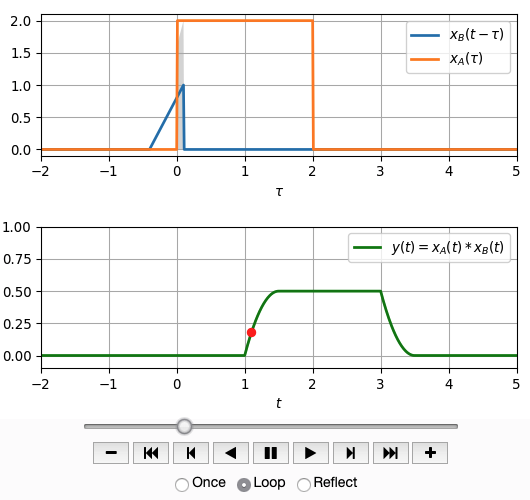
\includegraphics[width=\textwidth]{../convolution_ct/conv_var1_1_1D3D68B312.png}
\caption{Teilüberlappung vorn, also $y_1(t)$.}
\label{fig:1D3D68B312_v1_1}
\end{subfigure}
\begin{subfigure}{0.45\textwidth}
\centering
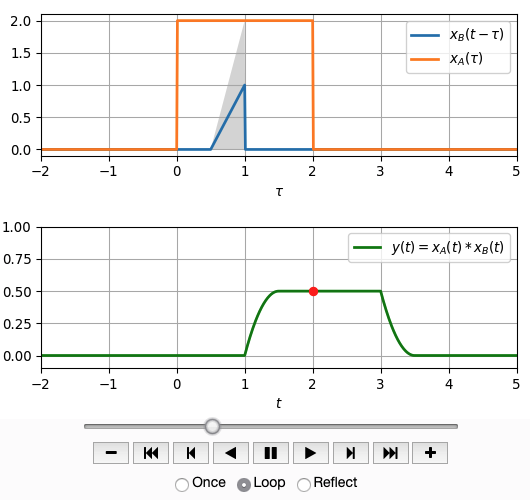
\includegraphics[width=\textwidth]{../convolution_ct/conv_var1_2_1D3D68B312.png}
\caption{Vollständige Überlappung, also $y_2(t)$.}
\label{fig:1D3D68B312_v1_2}
\end{subfigure}
\\
\begin{subfigure}{0.45\textwidth}
\centering
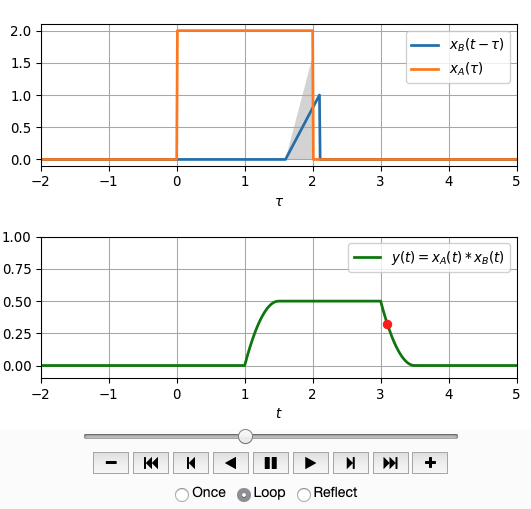
\includegraphics[width=\textwidth]{../convolution_ct/conv_var1_3_1D3D68B312.png}
\caption{Teilüberlappung hinten, also $y_3(t)$.}
\label{fig:1D3D68B312_v1_3}
\end{subfigure}
\begin{subfigure}{0.45\textwidth}
\centering
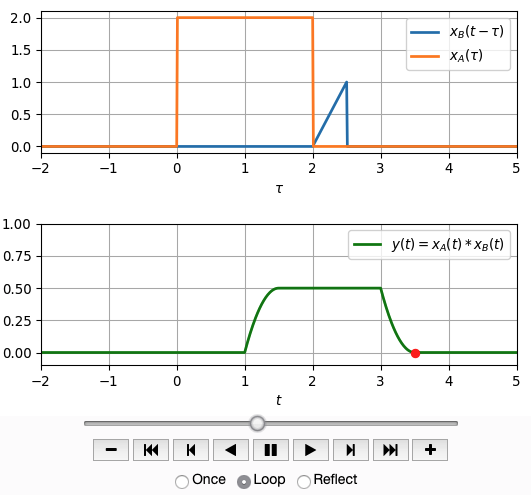
\includegraphics[width=\textwidth]{../convolution_ct/conv_var1_4_1D3D68B312.png}
\caption{Keine Überlappung hinten, also $y_4(t)$.}
\label{fig:1D3D68B312_v1_4}
\end{subfigure}
%
\caption{Faltungsprozess Variante I.
\texttt{convolution\_ct\_example1\_1D3D68B312.ipynb}}
\label{fig:1D3D68B312_v1}
\end{figure*}

\begin{ExCalc}
\textbf{Variante II: Zeitumkehr und Zeitverschiebung}  für $x(t)$
\begin{equation}
y(t) = \int\limits_{-\infty}^{+\infty} x(-\tau+t) h(\tau) \, \fsd \tau
\end{equation}
\begin{itemize}
  \item Schritt 1: Substitution $t\rightarrow \tau$ für $h(t)$
  \begin{equation}
  h(\tau) =
  \begin{cases}
  -2 \tau + 3 \quad \mathrm{für} \quad\red{1} \leq \tau \leq \red{\frac{3}{2}}\\
  0 \quad \mathrm{sonst}
  \end{cases}
  \end{equation}
  \item Schritt 2:  Substitution $t\rightarrow -\tau + t$ für $x(t)$
  \begin{equation}
  x(-\tau+t)=
  \begin{cases}
    2 \quad \mathrm{für} \quad 0 \leq -\tau+t \leq 2\\
    0 \quad \mathrm{sonst}
  \end{cases}
  \end{equation}
  \item Schritt 3:  Intervallgrenzen anpassen
  \begin{equation}
  x(-\tau+t)=
  \begin{cases}
    2 \quad \mathrm{für} \quad \blue{-2+t} \leq \tau \leq \blue{t}\\
    0 \quad \mathrm{sonst}
  \end{cases}
  \end{equation}
  \item Schritt 4: Stammfunktionansatz aufschreiben
  \begin{equation}
  y(t) =
  \int\limits_{a}^{b} x(-\tau+t) \cdot h(\tau) \fsd \tau =
  \int\limits_{a}^{b} 2 \cdot (-2 \tau + 3) \fsd \tau
  \end{equation}
  und berechnen zu
  \begin{equation}
  y(t) = -2 \tau^2 +6 \tau\bigg|_{\tau=a}^{\tau=b}
  \end{equation}
  Die \red{Intervall}\blue{grenzen} gehen als Integrationsbereiche $a,b$ in die Faltung ein.
  \item Schritt 5:  Signal-Überlappungen
  siehe Variante I
  % $x(t)$ ist endliches Signal von $t_1=0$ bis $t_2=2$
  %
  % $h(t)$ ist endliches Signal von $t_3=1$ bis $t_4=\frac{3}{2}$
  %
  % $y(t)$ wird daher ein endliches Signal von $t_1+t_3=1$ bis $t_2+t_4=\frac{7}{2}$ sein
  %
  % es gibt eine Teilüberlappung von $x(\tau)$ und $h(-\tau+t)$  'vorne' von
  % $t_1+t_3$ bis $t_1+t_3+T$
  %
  % es gibt eine Teilüberlappung von $x(\tau)$ und $h(-\tau+t)$  'hinten' von
  % $t_2+t_4-T$ bis $t_2+t_4$
  %
  % $T$ ist die Länge des kürzeren Signals, also hier $T=\frac{1}{2}$
  %
  % vollständige Überlappung hier für von $t = \frac{3}{2}$ bis $t=3$
  %
  % $y(t)=0$ für $t<(t_1+t_3)$ und $t\geq(t_2+t_4)$
  %
  % Diese Erkenntnisse in einer Formel
  % \begin{equation}
  % y(t) =
  % \begin{cases}
  %   y_1(t) \qquad \mathrm{für} \qquad 1 \leq t < \frac{3}{2}\\
  %   y_2(t) \qquad \mathrm{für} \qquad \frac{3}{2} \leq t < 3\\
  %   y_3(t) \qquad \mathrm{für} \qquad 3 \leq t < \frac{7}{2}\\
  %   y_4(t)=0 \qquad \mathrm{sonst}
  % \end{cases}
  % \end{equation}

  \item Schritt 6:  Stammfunktion mit Grenzen auswerten

  \begin{equation}
  y_1(t) = -2 \tau^2 +6 \tau\bigg|_{\tau=\red{1}}^{\tau=\blue{t}}
  = -2 t^2 + 6 t - 4
  \end{equation}

  \begin{equation}
  y_2(t) = -2 \tau^2 +6 \tau\bigg|_{\tau=\red{1}}^{\tau=\red{\frac{3}{2}}}  = \frac{1}{2}
  \end{equation}

  \begin{equation}
  y_3(t) = -2 \tau^2 +6 \tau\bigg|_{\tau=\blue{-2+t}}^{\tau=\red{\frac{3}{2}}} = +2 t^2 - 14 t + \frac{49}{2}
  \end{equation}

\end{itemize}
\end{ExCalc}

\begin{Loesung}
Das Ergebnis der Faltung, also das Ausgangssignal unseres LTI-Systems ist
wie erwartet gleich mit Variante I
\begin{align}
y(t) =
\begin{cases}
  y_1(t) = -2 t^2 + 6 t - 4 &\qquad \mathrm{für} \qquad 1 \leq t < \frac{3}{2}\\
  y_2(t) = \frac{1}{2}  &\qquad \mathrm{für} \qquad \frac{3}{2} \leq t < 3\\
  y_3(t) = +2 t^2 - 14 t + \frac{49}{2} &\qquad \mathrm{für} \qquad 3 \leq t < \frac{7}{2}\\
  y_4(t)=0 &\qquad \mathrm{sonst}
\end{cases}
\end{align}
Im Vergleich zu Variante I ist diese Lösung vielleicht
intuitiver, weil wir die Rechteckfunktion zeitlich verschieben und die
Integrallgrenzen schneller einleuchten.
%
Die Lösung wird in \fig{fig:1D3D68B312_v2} veranschaulicht für verschiedene
Zeiten $t$. In blau der zeitlich umgekehrte, verschobene Rechteckimpuls, in
orange die unverschobene Impulsantwort und in grün das Ausgangssignal der Faltung.
%
Wir sollten uns die \textbf{Unterschiede der Stammfunktionen und der Grenzen in den
Varianten I und II} genau anschauen.
Die Grenzen müssen stimmig sein zu der Funktion die verschoben wird.
%

Einem Rechteckimpuls sieht man nicht durch reines Hinschauen an, dass er
zeitlich gedreht wurde, hier ist also besondere Obacht erforderlich.
%
Gut gemeintes einfaches Integrieren erkaufen wir uns hier also mit tendenzieller
Verwirrung beim Signalspiegeln.
%
Erfahrungsgemäß braucht diese Rechnerei mal einen sehr ruhigen Moment und vertieftes
Sinnieren, während die Faltungsanimation in Dauerschleife läuft, irgendwann
wird klar, was wie verschoben werden muss und mit den Integrationsgrenzen verlinkt
ist.
%
\end{Loesung}















\begin{figure*}[h!]
\centering
\begin{subfigure}{0.45\textwidth}
\centering
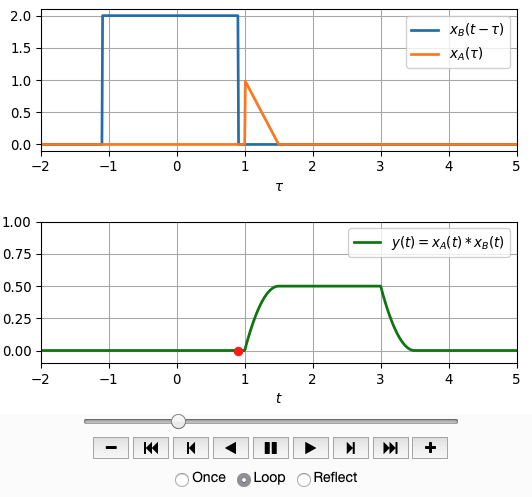
\includegraphics[width=\textwidth]{../convolution_ct/conv_var2_4_1D3D68B312.png}
\caption{Keine Überlappung vorne, also $y_4(t)$.}
\label{fig:1D3D68B312_v2_4}
\end{subfigure}
\begin{subfigure}{0.45\textwidth}
\centering
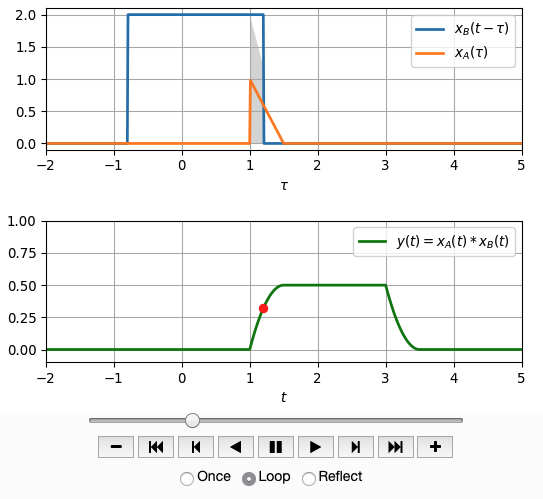
\includegraphics[width=\textwidth]{../convolution_ct/conv_var2_1_1D3D68B312.png}
\caption{Teilüberlappung vorn, also $y_1(t)$.}
\label{fig:1D3D68B312_v2_1}
\end{subfigure}
\\
\begin{subfigure}{0.45\textwidth}
\centering
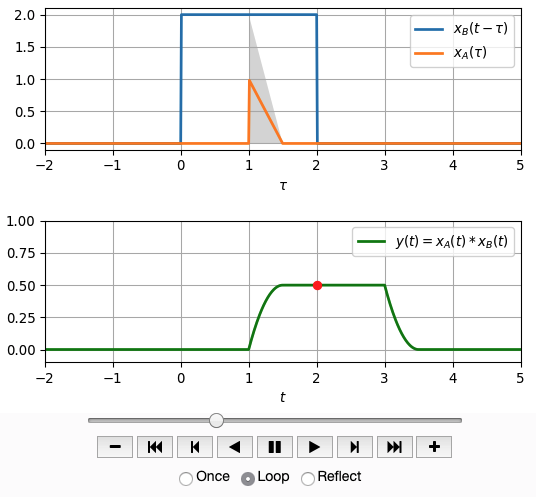
\includegraphics[width=\textwidth]{../convolution_ct/conv_var2_2_1D3D68B312.png}
\caption{Vollständige Überlappung, also $y_2(t)$.}
\label{fig:1D3D68B312_v2_2}
\end{subfigure}
\begin{subfigure}{0.45\textwidth}
\centering
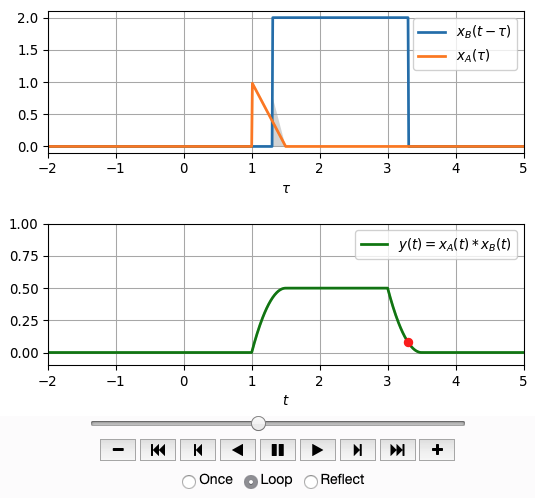
\includegraphics[width=\textwidth]{../convolution_ct/conv_var2_3_1D3D68B312.png}
\caption{Teilüberlappung hinten, also $y_3(t)$.}
\label{fig:1D3D68B312_v2_3}
\end{subfigure}
%
\caption{Faltungsprozess Variante II.
\texttt{convolution\_ct\_example1\_1D3D68B312.ipynb}}
\label{fig:1D3D68B312_v2}
\end{figure*}


\clearpage
\subsection{Faltung Rechteckimpuls mit Exponentialimpuls}
\label{sec:AF3B15E0D3}
\begin{Ziel}
Diese Aufgabe ist sehr ähnlich zu Aufgabe \ref{sec:1D3D68B312}.
Nur die Funktion von $h(t)$ ist verändert, alle Grenzen und
Längenbetrachtungen bleiben jedoch gleich. Das hat einen didaktischen
Hintergrund: Wir wollen hier zu der Erkenntnis kommen, dass eine exp()-Funktion
das Faltungsergebnis an den Sprungstellen anders 'glättet' als der Dreiecksimpuls
vorher.
Wenn wir $h(t)$ wieder als Impulsantwort eines LTI-System auffassen wollen,
heisst das, dass dieses System im Wesen ähnliche Dinge macht, aber im Detail
leicht anderes System-Verhalten hat.
\end{Ziel}
\textbf{Aufgabe} {\tiny AF3B15E0D3}: Berechnen Sie für die in der Skizze dargestellten
endlichen Signale $h(t)$ und $x(t)$ die Faltung $y(t)=x(t) \ast h(t)$.

\begin{tikzpicture}
\begin{axis}[
width=0.5\textwidth,
height=0.3\textwidth,
domain=1:3/2,
samples=20,
legend pos=outer north east,
xlabel = {t / s},
ylabel = {h(t), x(t)},
xmin=-1, xmax=4,
ymin=-0.1, ymax=2.1,
xtick={0,1,1.5,2},
ytick={0,1,2},
ymajorgrids=true,
xmajorgrids=true
]
\addplot[mark=None, color=C1, ultra thick] {exp(-6*(x-1))};
\addplot[mark=None, color=C0, ultra thick]
coordinates {(-1,0)(0,0)(0,2)(2,2)(2,0)(4,0)};
\addplot[mark=None, color=C1, ultra thick]
coordinates {(-1,0)(1,0)(1,1)};
\addplot[mark=None, color=C1, ultra thick]
coordinates {(1.5,0.05)(1.5,0)(4,0)};
\legend{$h(t)=\exp(-[t-1] \cdot 6) \cdot \mathrm{rect}([t-\frac{5}{4}] \cdot 2)$,
$x(t)=2\,\mathrm{rect}([t-1]\cdot \frac{1}{2})$}
\end{axis}
\end{tikzpicture}



\begin{Werkzeug}
Es ist mutmaßlich schöner zu integrieren, wenn wir $x(t)$ zeitlich umkehren und
verschieben, daher
\begin{equation}
y(t) = \int\limits_{-\infty}^{+\infty} x(-\tau+t) h(\tau) \, \fsd \tau
\end{equation}
also analog zur wahrscheinlich zugänglicheren Variante II aus Aufgabe
\ref{sec:1D3D68B312}.
\end{Werkzeug}


\begin{Ansatz}
Signale so darstellen, das wir den stückweisen Verlauf in seinen Grenzen angeben können.
Also: die Exponentialfunktion zeitlich verzögert um 1, schneller abfallend heißt zeitlich
gestaucht, Faktor 6
\begin{equation}
h(t) =
\begin{cases}
\e^{-[t-1]\cdot 6} \quad \mathrm{für} \quad 1 \leq t \leq \frac{3}{2}\\
0 \quad \mathrm{sonst}
\end{cases}
\end{equation}
Und der schon bekannte Rechteckimpuls
\begin{equation}
x(t)=
\begin{cases}
  2 \quad \mathrm{für} \quad 0 \leq t \leq 2\\
  0 \quad \mathrm{sonst}
\end{cases}
\end{equation}
Fassen wir $h(t)$ wieder als Impulsantwort eines LTI-Systems und $x(t)$ als
Eingangssignal in dieses auf. Wir werden gleich sehen, dass wir mit der Denke
sehr nah an der Praxis sind.
\end{Ansatz}




\begin{ExCalc}
Wir benutzen
\textbf{Variante II: Zeitumkehr und Zeitverschiebung}  für $x(t)$
\begin{equation}
y(t) = \int\limits_{-\infty}^{+\infty} x(-\tau+t) h(\tau) \, \fsd \tau
\end{equation}
und folgen unserem Algorithmus:
\begin{itemize}
  \item Schritt 1: Substitution $t\rightarrow \tau$ für $h(t)$
  \begin{equation}
  h(\tau) =
  \begin{cases}
  \e^{-[\tau-1]\cdot 6} \quad \mathrm{für} \quad\red{1} \leq \tau \leq \red{\frac{3}{2}}\\
  0 \quad \mathrm{sonst}
  \end{cases}
  \end{equation}
  \item Schritt 2:  Substitution $t\rightarrow -\tau + t$ für $x(t)$
  \begin{equation}
  x(-\tau+t)=
  \begin{cases}
    2 \quad \mathrm{für} \quad 0 \leq -\tau+t \leq 2\\
    0 \quad \mathrm{sonst}
  \end{cases}
  \end{equation}
  \item Schritt 3:  Intervallgrenzen anpassen
  \begin{equation}
  x(-\tau+t)=
  \begin{cases}
    2 \quad \mathrm{für} \quad \blue{-2+t} \leq \tau \leq \blue{t}\\
    0 \quad \mathrm{sonst}
  \end{cases}
  \end{equation}
  \item Schritt 4: Stammfunktionansatz
  \begin{equation}
  y(t) =
  \int\limits_{a}^{b} x(-\tau+t) \cdot h(\tau) \fsd \tau =
  \int\limits_{a}^{b} 2 \cdot (\e^{-[\tau-1]\cdot 6}) \fsd \tau
  \end{equation}
  und berechnen zu (auch noch ein eher triviales Integral)
  \begin{equation}
  y(t) = -\frac{1}{3}\e^{-[\tau-1]\cdot 6}\bigg|_{\tau=a}^{\tau=b}
  \end{equation}
  Die \red{Intervall}\blue{grenzen} gehen als Integrationsbereiche $a,b$ in die Faltung ein.

  \item Schritt 5:  Signal-Überlappungen

  $x(t)$ ist endliches Signal von $t_1=0$ bis $t_2=2$

  $h(t)$ ist endliches Signal von $t_3=1$ bis $t_4=\frac{3}{2}$

  $y(t)$ wird daher ein endliches Signal von $t_1+t_3=1$ bis $t_2+t_4=\frac{7}{2}$ sein

  es gibt eine Teilüberlappung von $x(\tau)$ und $h(-\tau+t)$  'vorne' von
  $t_1+t_3$ bis $t_1+t_3+T$

  es gibt eine Teilüberlappung von $x(\tau)$ und $h(-\tau+t)$  'hinten' von
  $t_2+t_4-T$ bis $t_2+t_4$

  $T$ ist die Länge des kürzeren Signals, also hier $T=\frac{1}{2}$

  vollständige Überlappung hier für von $t = \frac{3}{2}$ bis $t=3$

  $y(t)=0$ für $t<(t_1+t_3)$ und $t\geq(t_2+t_4)$

  Diese Erkenntnisse in einer Formel
  \begin{equation}
  y(t) =
  \begin{cases}
    y_1(t) \qquad \mathrm{für} \qquad 1 \leq t < \frac{3}{2}\\
    y_2(t) \qquad \mathrm{für} \qquad \frac{3}{2} \leq t < 3\\
    y_3(t) \qquad \mathrm{für} \qquad 3 \leq t < \frac{7}{2}\\
    y_4(t)=0 \qquad \mathrm{sonst}
  \end{cases}
  \end{equation}

  \item Schritt 6:  Stammfunktion mit Grenzen auswerten

  \begin{equation}
  y_1(t) = -\frac{1}{3}\e^{-[\tau-1]\cdot 6}\bigg|_{\tau=\red{1}}^{\tau=\blue{t}}
  = \frac{1}{3}\left(1-\e^{-[t-1] \cdot 6}\right)
  \end{equation}

  \begin{equation}
  y_2(t) = -\frac{1}{3}\e^{-[\tau-1]\cdot 6}\bigg|_{\tau=\red{1}}^{\tau=\red{\frac{3}{2}}}  =
  \frac{1}{3}\left(1-\e^{-3}\right) \approx 0.316737...
  \end{equation}

  \begin{equation}
  y_3(t) = -\frac{1}{3}\e^{-[\tau-1]\cdot 6}\bigg|_{\tau=\blue{-2+t}}^{\tau=\red{\frac{3}{2}}} =
  \frac{1}{3}\left(\e^{-[t-3] \cdot 6} - \e^{-3}\right)
  \end{equation}
\end{itemize}
\end{ExCalc}


\begin{Loesung}
Das gesuchte Faltungsergebnis ist also
\begin{align}
y(t) =
\begin{cases}
  y_1(t) = \frac{1}{3}\left(1-\e^{-[t-1] \cdot 6}\right) &\qquad \mathrm{für} \qquad 1 \leq t < \frac{3}{2}\\
  y_2(t) = \frac{1}{3}\left(1-\e^{-3}\right) \approx 0.316737 &\qquad \mathrm{für} \qquad \frac{3}{2} \leq t < 3\\
  y_3(t) = \frac{1}{3}\left(\e^{-[t-3] \cdot 6} - \e^{-3}\right) &\qquad \mathrm{für} \qquad 3 \leq t < \frac{7}{2}\\
  y_4(t)=0 &\qquad \mathrm{sonst}
\end{cases}
\end{align}

In \fig{fig:AF3B15E0D3_v2} ist der Faltungsprozess veranschaulicht.
%
Stellen wir im Vergleich zu Aufgabe \ref{sec:1D3D68B312} fest, dass
%
\begin{itemize}
  \item die Grenzen für Signalabschnitte gleich geblieben sind (diese Aufgabe war ja so
  ausgelegt)
  \item $y_2(t)$ wieder ein konstanten Verlauf hat, nur diesmal mit der Amplitude von ca.
  $0.316737$. Die Fläche des Exponentialimpulses ist ja kleiner als die des Dreickimpulses
  aus Aufgabe \ref{sec:1D3D68B312}
  \item die Gleichungen, welche die stückweisen Abschnitte definieren diesmal mit der
  Exponentialfunktion beschrieben werden. Auch das sollte wieder einleuchten,
  beim Integrieren einer Exponentialfunktion resultiert wieder eine Exponentialfunktion
\end{itemize}
%
\textbf{Ladekurven Kondensator?!?} Wenn wir uns das Faltungsergebnis $y(t)$
(grüner Graph) und die Ergebnisgleichungen anschauen, wird uns
vielleicht eine verblüffende Ähnlichkeit zu Auf-/Entladekurven eines
RC-Gliedes auffallen. Wir schauen uns das in der nächsten Aufgabe \ref{sec:C964DD7400}
genauer an. Hier schon mal soviel, es ist sehr ähnlich aber nicht exakt identisch.
Der Grund liegt in der hier betrachteten \textbf{endlichen} Impulsantwort. Ein
RC-Glied hat eine \textbf{unendliche} Impulsantwort.
\end{Loesung}


\begin{figure*}[h!]
\centering
\begin{subfigure}{0.45\textwidth}
\centering
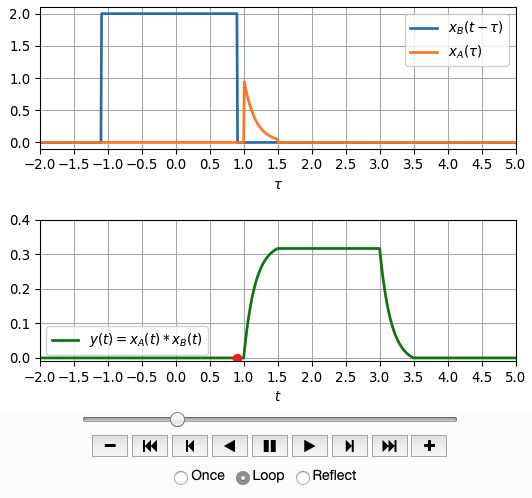
\includegraphics[width=\textwidth]{../convolution_ct/conv_var2_4_AF3B15E0D3.png}
\caption{Keine Überlappung vorne, also $y_4(t)$.}
\label{fig:AF3B15E0D3_v2_4}
\end{subfigure}
\begin{subfigure}{0.45\textwidth}
\centering
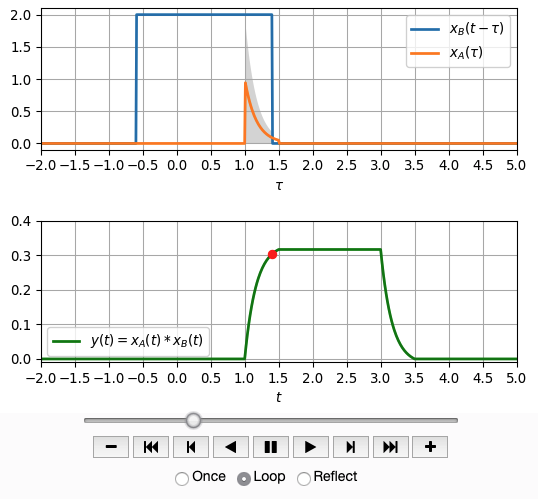
\includegraphics[width=\textwidth]{../convolution_ct/conv_var2_1_AF3B15E0D3.png}
\caption{Teilüberlappung vorn, also $y_1(t)$.}
\label{fig:AF3B15E0D3_v2_1}
\end{subfigure}
\\
\begin{subfigure}{0.45\textwidth}
\centering
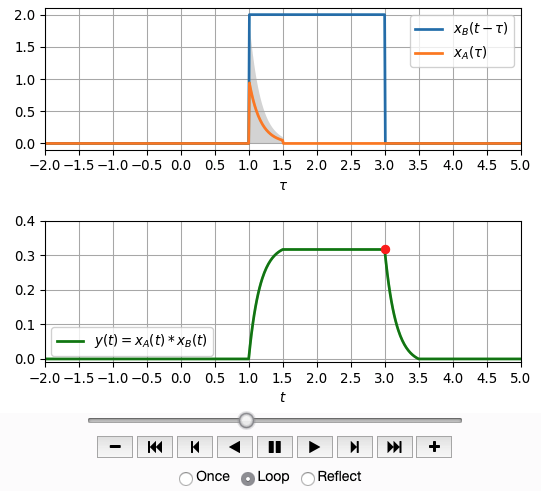
\includegraphics[width=\textwidth]{../convolution_ct/conv_var2_2_AF3B15E0D3.png}
\caption{Vollständige Überlappung, also $y_2(t)$.}
\label{fig:AF3B15E0D3_v2_2}
\end{subfigure}
\begin{subfigure}{0.45\textwidth}
\centering
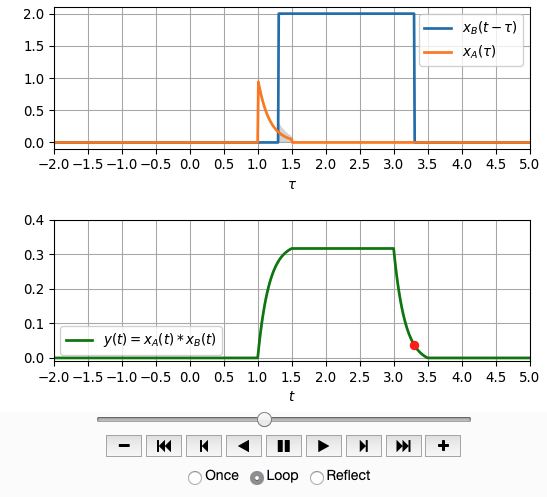
\includegraphics[width=\textwidth]{../convolution_ct/conv_var2_3_AF3B15E0D3.png}
\caption{Teilüberlappung hinten, also $y_3(t)$.}
\label{fig:AF3B15E0D3_v2_3}
\end{subfigure}
%
\caption{Faltungsprozess Aufgabe \ref{sec:AF3B15E0D3}.
\texttt{convolution\_ct\_example2\_AF3B15E0D3.ipynb}}
\label{fig:AF3B15E0D3_v2}
\end{figure*}



\clearpage
\subsection{Faltung Rechteckimpuls mit Exponentialfunktion}
\label{sec:C964DD7400}
\begin{Ziel}
Wir werden anhand einer speziellen Faltung eines endlichen Signals mit
einem unendlichen Signal, einen ganz fundamentalen Link zur Elektrotechnik
und DGLs 1. Ordnung mit konstanten Koeffizienten herstellen:
Sprungartige Spannungsänderungen an passiven Energiespeichern (Auf-/Entladen) können wir
sehr elegant mit Signal-und Systemtheorie Werkzeugen berechnen. Es wird mit
der Laplace Transformation später sogar noch eleganter.
\end{Ziel}
\textbf{Aufgabe} {\tiny C964DD7400}: Für das unten abgebildete RC-Glied
(Annahme: ideale Bauelemente)
gilt die \textbf{Impulsantwort} (wir nehmen LTI System-Eigenschaften an)
\begin{equation}
h(t) = \frac{1}{T_\mathrm{RC}} \cdot \e^{-\frac{t}{T_\mathrm{RC}}}
\qquad \mathrm{für} \qquad t \geq 0
\qquad \mathrm{mit} \qquad T_\mathrm{RC} = R \cdot C
\end{equation}
Wir betrachten das RC-Glied als ruhend, also $y(0)=0$.
%
Berechnen Sie für $T_\mathrm{RC}=\frac{1}{5}$ s und für das unten dargestellte
Eingangssignal $x(t)$ das Faltungsergebnis $y(t)=x(t) \ast h(t)$.
%
\begin{center}
\begin{circuitikz}[european, scale=0.75]
\node (in) at (1,0){};
\node (in_ground) at (1,-3){};
\node (out) at (4,0){};
\node (out_ground) at (4,-3){};
\draw (in) to [R,l_=$R$,o-] (3,0);
\draw (3,0) to [short,-o,] (out);
\draw (3,0) to [C,l_=$C$,*-*] (3,-3);
\draw (in_ground) to [short,o-o] (out_ground);
\path[draw, bend right, ->, >=latex] (in) edge node[left]{Eingangsspannung $x(t)$} (in_ground);
\path[draw, bend left, ->, >=latex] (out) edge node[right]{Ausgangsspannung $y(t)$} (out_ground);
\end{circuitikz}
\end{center}
%
\begin{tikzpicture}
\begin{axis}[
width=0.5\textwidth,
height=0.3\textwidth,
domain=0:4,
samples=50,
legend pos=outer north east,
xlabel = {t / s},
ylabel = {h(t), x(t)},
xmin=-1, xmax=4,
ymin=-0.1, ymax=1.1,
xtick={0,1,2,3},
ytick={0,0.5,1,1.5,2},
ymajorgrids=true,
xmajorgrids=true
]
\addplot[mark=None, color=C0, ultra thick]
coordinates {(-1,0)(0,0)(0,1)(2,1)(2,0)(4,0)};
\addplot[mark=None, color=C1, ultra thick]
coordinates {(-1,0)(0,0)(0,1)};
\addplot[mark=None, color=C1, ultra thick] {exp(-5*(x))};
\legend{$x(t)=\mathrm{rect}([t-1]\cdot \frac{1}{2})$,
$\frac{1}{5} \cdot h(t)=\exp(- t \cdot 5) \cdot \epsilon(t)$}
\end{axis}
\end{tikzpicture}

\noindent\textbf{Hinweis 1}: Wir werden nach der Übung~\ref{sec:ue3_laplace} (3) in der Lage sein, $h(t)$ elegant herzuleiten.
Nehmen wir das an dieser Stelle mal hin, aber bemerken auch, dass wir
diese Art Formel beim Kondensator eh schon mal gesehen haben, mutmaßlich aber
nicht im Kontext einer Impulsantwort.

\noindent\textbf{Hinweis 2}: In der Elektrotechnik verwenden wir gerne $\tau$ für die Zeitkonstante. Weil das
aber unsere Hilfsvariable in der Faltung ist, geben wir der Zeitkonstante des RC-Glieds die Variable
$T_\mathrm{RC}$.

\noindent\textbf{Hinweis 3}: Aufgabe \ref{sec:AF3B15E0D3} behandelte den \textbf{endlichen Exponentialimpuls}
mit einer Zeitkonstante $1/6$ s, hier verwenden wir die abfallende Exponentialfunktion
die sich nur asymptotisch gegen Null nähert, die also eine \textbf{unendliche Impulsantwort}
darstellt. Der schöneren Anschauung wegen, wählen wir $T_\mathrm{RC}=1/5$ s, weil
dann bei 1 s zu 99\% der finale Lade-/Entlade-Amplitudenwert erreicht ist
(vgl. $5 T_\mathrm{RC}$-Regel).

\noindent\textbf{Hinweis 4}: Machen wir uns noch klar, dass wir es hier mit der DGL 1. Ordnung
mit konstanten Koeffizienten
\begin{equation}
T_\mathrm{RC} \frac{\fsd y(t)}{\fsd t} + y(t) = x(t)
\end{equation}
mit $y(0)=0$ zu tun haben und überlegen, wie wir die Aufgabe mit
typischem Mathe-DGL Handwerk lösen würden. Siehe auch SigSys-Klausur WS19/20 Aufgabe 1.

\begin{Werkzeug}
Es ist mutmaßlich wieder schöner zu integrieren,
wenn wir $x(t)$ zeitlich umkehren und verschieben, daher Faltungsintegral
\begin{equation}
y(t) = \int\limits_{-\infty}^{+\infty} x(-\tau+t) h(\tau) \, \fsd \tau
\end{equation}

\end{Werkzeug}
\begin{Ansatz}
Die Signale zum Falten sind
\begin{equation}
h(t) =
\begin{cases}
\frac{1}{\frac{1}{5}} \e^{-\frac{t}{\frac{1}{5}}} = 5 \e^{-5 t} \quad \mathrm{für} t \geq 0\\
0 \quad \mathrm{sonst}
\end{cases}
\end{equation}
\begin{equation}
x(t)=
\begin{cases}
  1 \quad \mathrm{für} \quad 0 \leq t \leq 2\\
  0 \quad \mathrm{sonst}
\end{cases}
\end{equation}
\end{Ansatz}

\begin{ExCalc}
Wir benutzen
\textbf{Variante II: Zeitumkehr und Zeitverschiebung}  für $x(t)$
\begin{equation}
y(t) = \int\limits_{-\infty}^{+\infty} x(-\tau+t) h(\tau) \, \fsd \tau
\end{equation}
Wir können diesmal nicht unseren bereits etablierten Algorithmus verwenden, weil
der nur funktioniert, wenn beide Signale endliche Länge haben.
%
Machen wir uns hier stattdessen zu nutze, dass die Rechteckfunktion durch zwei
Sprungfunktionen dargestellt werden kann, nämlich $x(t) = \epsilon(t) - \epsilon(t-2)$.
%
Es gilt das Superpositionsprinzip bei LTI-Systemen. Daher
können wir für die beiden einzelnen Sprünge die Faltungen einzeln ausrechnen.
%
Das gelingt besonders elegant, wenn man für die Faltung die Sprünge als die
zeitumgekehrten und verschobenen Signale auffasst (damit wäre Klausuraufgabe 1
vom SS2019 ganz schnell berechnet).
%
Konkret also: Faltung mit der Sprungfunktion $x_1(t) = \epsilon(t)$ führt auf
\begin{equation}
y_1(t) = \int\limits_{0}^{t} 1 \cdot 5 \e^{- 5 \tau} \fsd \tau= \left(1-\e^{-5 t}\right)
\qquad \mathrm{für} \qquad t \geq 0
\end{equation}
%
Faltung mit der Sprungfunktion $x_2(t) = -\epsilon(t-2)$ führt auf
\begin{equation}
y_2(t) =
\begin{cases}
  0 &\qquad \mathrm{für} \qquad t < 2\\
  \int\limits_{2}^{t} -1 \cdot 5 \e^{- 5 [\tau-2]}  \fsd \tau = \left( \e^{-5 [t-2]}-1\right) &\qquad \mathrm{für} \qquad t \geq 2
\end{cases}
\end{equation}
%
% Bitte nochmal mit Wolfram Alpha gegenchecken:
% Ansatz für gedrehte Impulsantwort
% integrate -step(tau-2)*5*exp(5*tau-5*t) d tau from 0 to t
% oder Ansatz für gedrehten Reckteckimpuls
% integrate -step(-tau+t-2)*5*exp(-5*tau) d tau from 0 to t

% Mit dem zweiteren, hab ich dann für 2.217 die beiden Funktionen verschoben (bzgl. tau) und die Integralgrenzen angepasst
% integrate -step(-tau+t)*5*exp(-5*(tau-2)) d tau from 2 to t
% und wenn wir dann explizit erwähnen, dass y(t) nur für t>=2, brauchen wir die step funktion im Integral nicht mehr und wir können mit dem Integral
% integrate -5*exp(-5*(tau-2)) d tau from 2 to t
% rechnen.
% %
% Es gilt das Superpositionsprinzip bei LTI-Systemen, also einer Eingangssumme
% $x(t) = x_1(t) + x_2(t) = \epsilon(t) - \epsilon(t-2)$
% folgt die Ausgangssumme $y(t) = y_1(t) + y_2(t)$.
\end{ExCalc}

\begin{Loesung}
Das Endergebnis lautet mit Superposition
\begin{equation}
y(t) = y_1(t) + y_2(t) =
  \begin{cases}
  \left(1-\e^{-5 t}\right) &\qquad \mathrm{für} \qquad 0 \leq t < 2\\
  \left(1-\e^{-5 t}\right) + \left( \e^{-5 [t-2]}-1\right) = \e^{-5 [t-2]} - \e^{-5 t}
  &\qquad \mathrm{für} \qquad t \geq 2
  \end{cases}
\end{equation}
und wir erkennen im ersten Teil der Gleichung die typische Aufladekurve des
Kondensators. Im zweiten Teil ist die nicht ganz so offensichtliche Entladekurve
zu sehen, wir entladen erst zum Zeitpunkt $t=2$ s, das muss in der exp()-Funktion
als Zeitverschiebung mit berücksichtigt werden.
%
Die gewählte Zeitkonstante ist sehr kurz im Vergleich zum Rechtecklänge, daher
kann man für den Kondensator mit guter Näherung drei Zustände während des
Anlegens von $x(t)$ definieren:
\begin{itemize}
  \item für $0<t<1$ Aufladen
  \item für $1<t<2$ Geladen
  \item für $2<t<3$ Entladen
\end{itemize}
Wie oben schon erwähnt, erfolgt vollständiges Aufladen und Entladen mit asymptotischer
Annäherung an den Endzustand.

Spannende Frage zum Sinnieren oder vielleicht sogar Rechnen:
Wie schaut das Ausgangssignal $y(t)$ aus, wenn man den Rechtecksprung sehr,
sehr, sehr kurz macht und vielleicht sogar Fläche 1 sicherstellt?

Spannender Link I: Wir haben mit
\begin{align}
y_1(t) =
\begin{cases}
1-\e^{-5 t} \quad \text{für} \quad t\geq 0\\
0 \quad \text{sonst}
\end{cases}
\end{align}
die sogenannte \textbf{Sprungantwort} $h_\epsilon(t)$ des Systems berechnet,
sozusagen als Abfallprodukt, weil wir die Sprungfunktion als Systemeingang gewählt
haben, und das System eben antwortet mit der ... Sprungantwort.

Spannender Link II: Die \textbf{Impulsantwort} $h(t)$ ist direkt proportional zur
Entladekurve eines Kondensators, wenn der Kondensator zum Zeitpunkt $t=0$
vollständig auf $U_q$ aufgeladen war und ab $t=0+$ die Entladung erfolgt.
Aus der Elektrotechnik wissen wir, dass dann $y(t) = U_q \e^{-\tau/T_\mathrm{RC}}$ gilt,
wir sehen Ähnlichkeiten mit $h(t) = \frac{1}{T_\mathrm{RC}} \cdot \e^{-\frac{t}{T_\mathrm{RC}}}$...

Wir bekommen langsam ein Gespür für die größeren Zusammenhänge und
warum SigSys nützlich sein könnte.
\end{Loesung}


\begin{figure*}[h!]
\centering
\begin{subfigure}{0.45\textwidth}
\centering
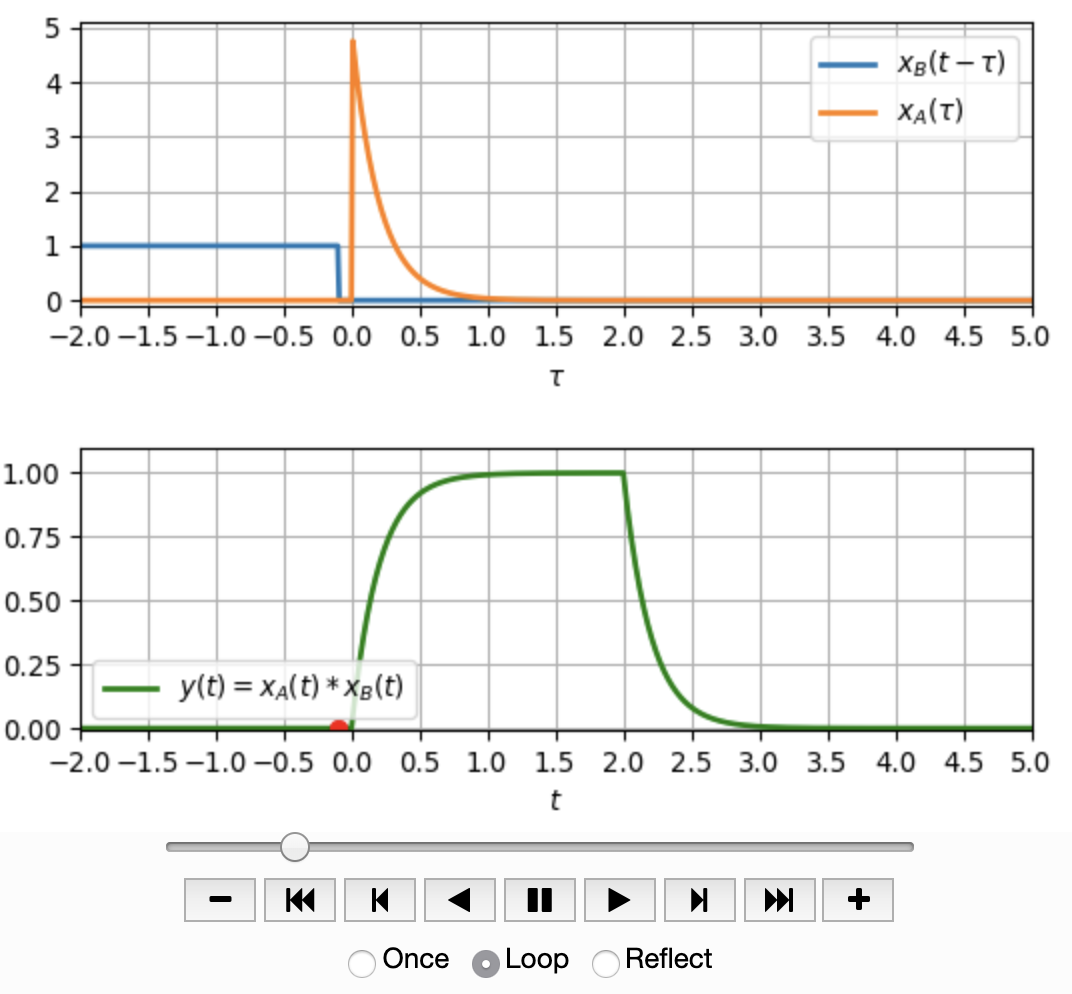
\includegraphics[width=\textwidth]{../convolution_ct/conv_var2_1_C964DD7400.png}
\caption{Keine Überlappung vorne.}
\label{fig:C964DD7400_v2_1}
\end{subfigure}
\begin{subfigure}{0.45\textwidth}
\centering
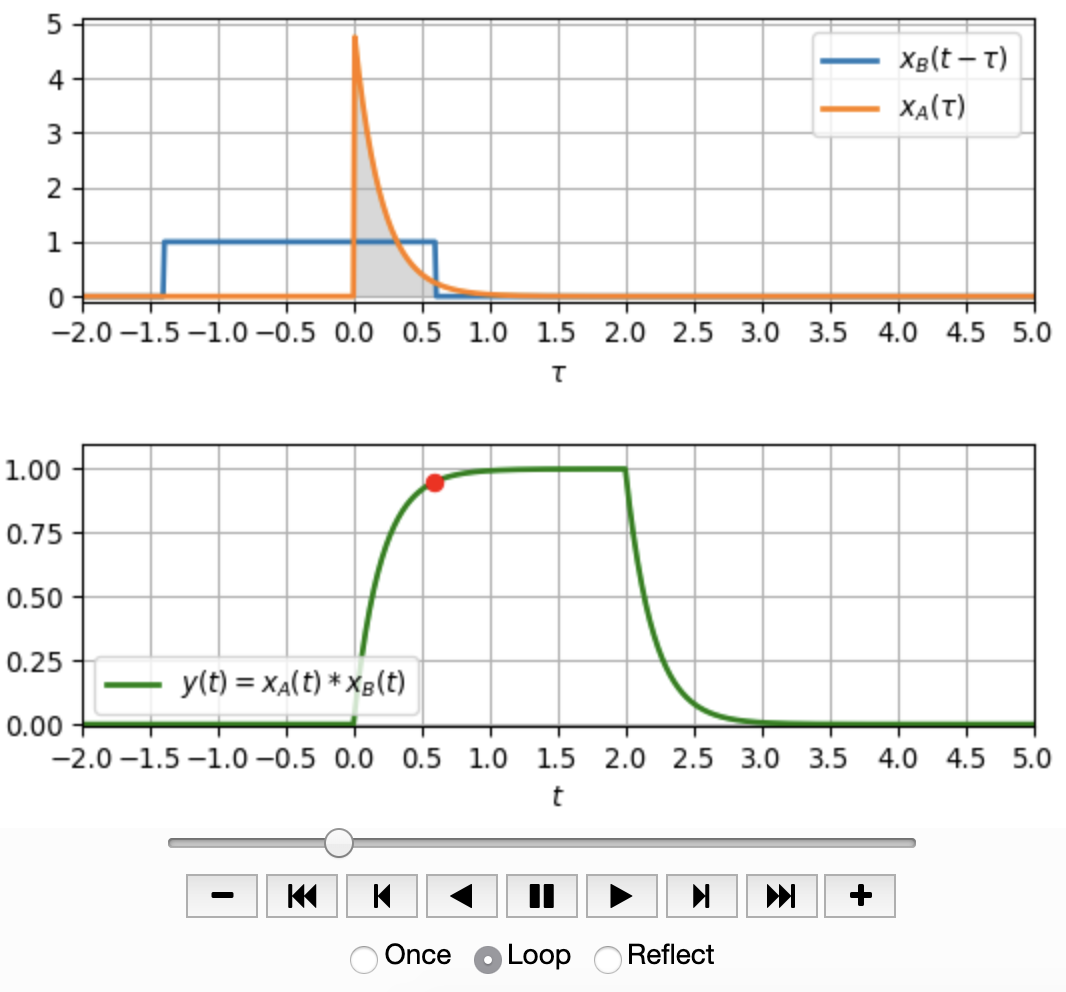
\includegraphics[width=\textwidth]{../convolution_ct/conv_var2_2_C964DD7400.png}
\caption{Teilüberlappung, Ladezustand: 95\%.}
\label{fig:C964DD7400_v2_2}
\end{subfigure}
\\
\begin{subfigure}{0.45\textwidth}
\centering
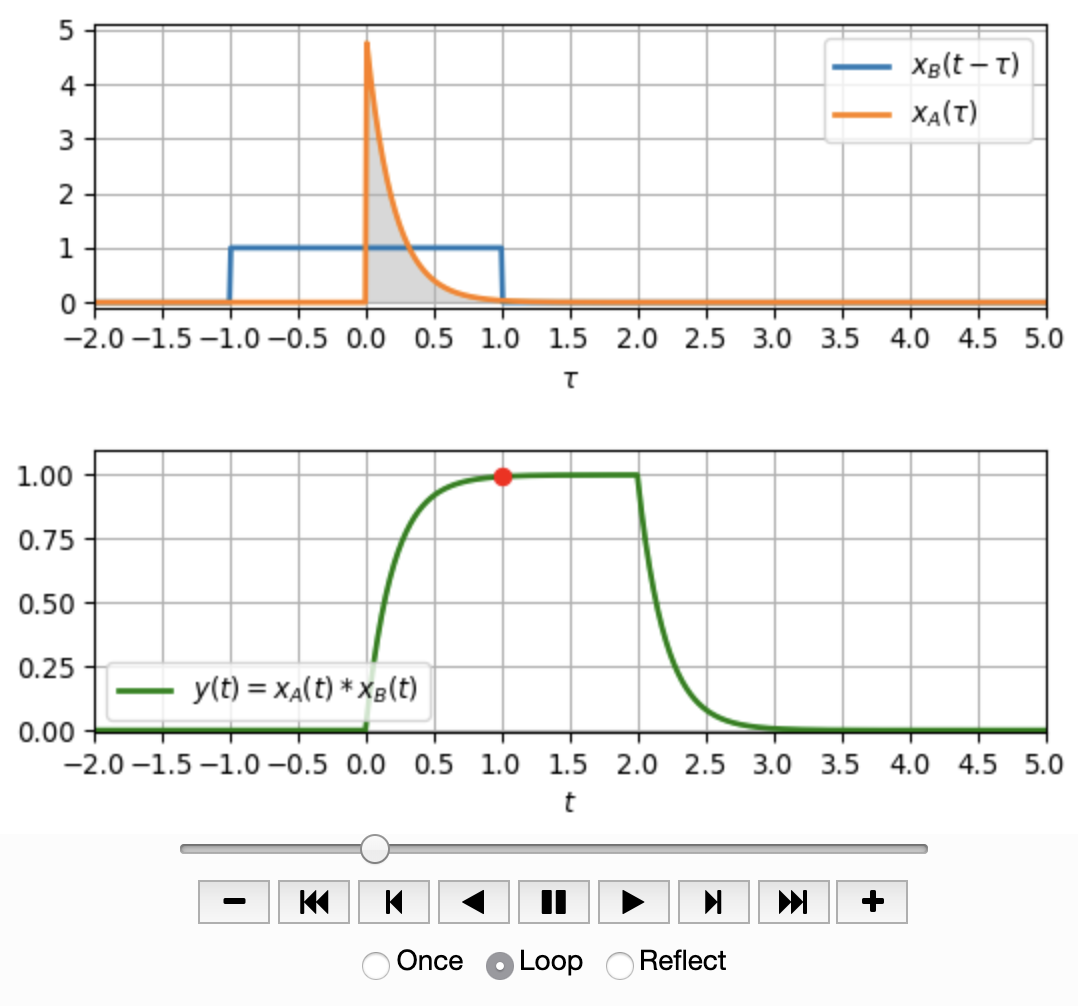
\includegraphics[width=\textwidth]{../convolution_ct/conv_var2_3_C964DD7400.png}
\caption{Teilüberlappung, Ladezustand: 99\%.}
\label{fig:C964DD7400_v2_3}
\end{subfigure}
\begin{subfigure}{0.45\textwidth}
\centering
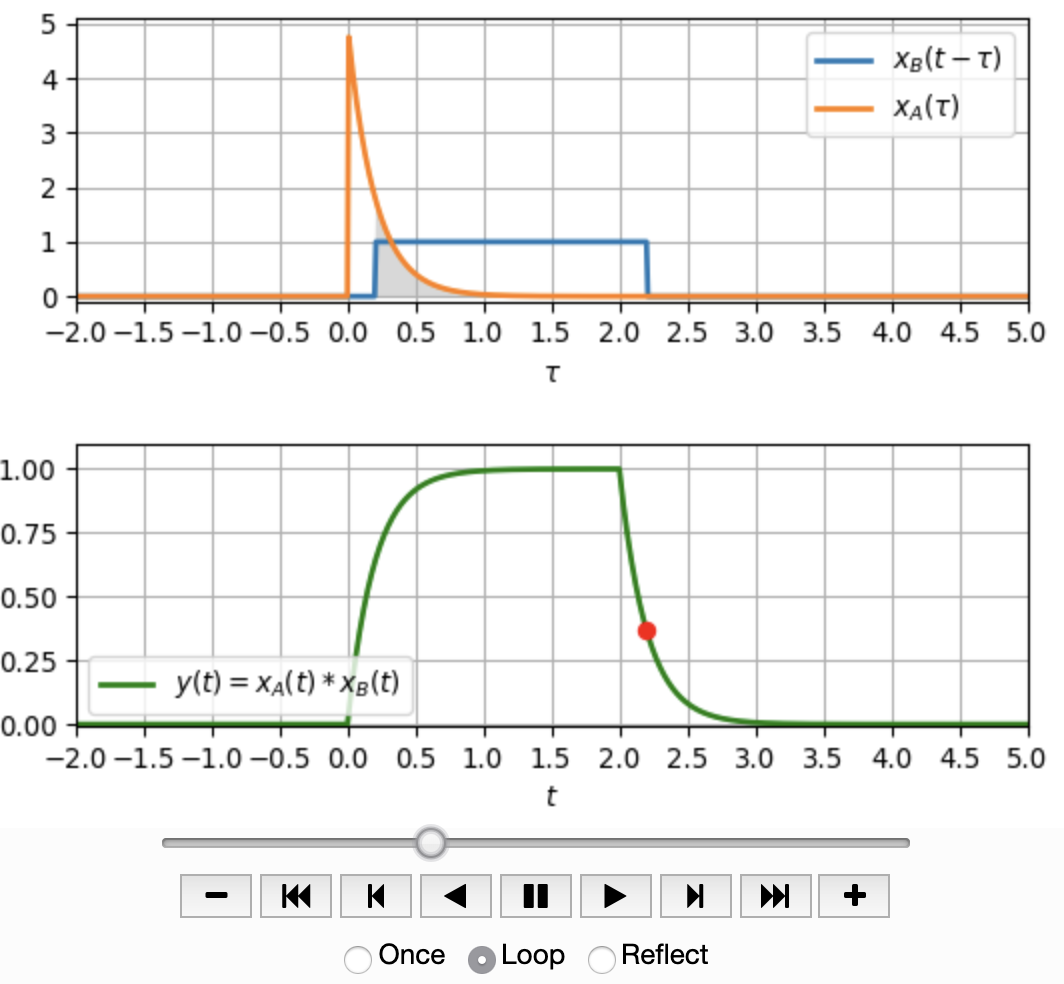
\includegraphics[width=\textwidth]{../convolution_ct/conv_var2_4_C964DD7400.png}
\caption{Teilüberlappung, Ladezustand: 37\% .}
\label{fig:C964DD7400_v2_4}
\end{subfigure}
%
\caption{Faltungsprozess Aufgabe \ref{sec:C964DD7400}.
\texttt{convolution\_ct\_example3\_C964DD7400.ipynb}}
\label{fig:C964DD7400_v2}
\end{figure*}
